\documentclass{article}

\usepackage{xeCJK}
\usepackage{amsfonts,amssymb}
\usepackage{amsmath}
\usepackage{geometry}
\usepackage{color}
\usepackage{graphicx}

\geometry{a4paper,scale=0.8}
\geometry{a4paper,left=3.18cm,right=3.18cm,top=2.54cm,bottom=2.54cm}
\linespread{1.5}

\definecolor{userColor}{RGB}{225,144,52}

\title{Consensus Problems in Networks of Agents\\ with Switching Topology and Time-Delays}
\author{ Jichao Zhao\thanks{E-mail: zhaojichao@imakerlab.cn}}
\date{25-10-2020}

% 正文开始
\begin{document}
\maketitle
% 生成目录
\tableofcontents


\begin{abstract}
In this paper, we discuss consensus problems for a network of dynamic agents with fixed and switching topologies. 
We analyze three cases: i) networks with switching topology and no time-delays, ii) networks with fixed topology and communication time-delays, and iii) max-consensus problems (or leader determination) for groups of discrete-time agents. 
In each case, we introduce a linear/nonlinear consensus protocol and provide convergence analysis for the proposed distributed algorithm. 
Moreover, we establish a connection between the Fiedler eigenvalue of the information flow in a network (i.e. algebraic connectivity of the network) and the negotiation speed (or performance) of the corresponding agreement protocol. 
It turns out that balanced digraphs play an important role in addressing average-consensus problems. 
We introduce disagreement functions that play the role of Lyapunov functions in convergence analysis of consensus protocols. 
A distinctive feature of this work is to address consensus problems for networks with directed information flow. 
We provide analytical tools that rely on algebraic graph theory, matrix theory, and control theory. 
Simulations are provided that demonstrate the effectiveness of our theoretical results.

这篇文章,我们讨论了动态智能体网络在固定和切换拓扑下的一致性问题。
我们分析了三种情况:i)切换拓扑无时延网络,ii)固定拓扑有时延网络,iii)智能体群离散时间下的的最大一致性问题(或领导力问题)。
在每一种情况,我们都介绍了线性/非线性的一致性协议,并且提供了分布式建议算法的收敛性分析。
此外,我们还建立了网络信息流的费德勒特征值(Fiedler eigenvaue)(即网络的代数连通度)和响应一致协议的收敛速度(或性能)之间的联系。
这表明平衡图在解决一致性问题上扮演着重要角色。
我们介绍了在一致性协议的收敛性分析问题中扮演着李雅普诺夫(Lyapunov functions)函数的非一致函数。
这项研究的显著特征是解决了有向信息流网络的一致性问题。
我们提供的分析工具基于代数图论,矩阵论和控制论。
仿真部分提供了我们的理论结果的演示效率。
\end{abstract}

\section{Introduction}
Distributed decision-making for coordination of networks of dynamic agents has attracted several researchers in recent years. 
This is partly due to broad applications of multi-agent systems in many areas including cooperative control of unmanned air vehicles (UAVs), flocking of birds [22, 24, 23], schooling for underwater vehicles, distributed sensory networks, attitude alignment of clusters of satellites, and congestion control in communication networks [21].

\noindent 这些年,动态智能体网络的分布式决策协调问题吸引了大量的研究者。
部分原因是因为多智能体系统(MAS)在许多领域都有广阔的应用,包括无人协同装置,类鸟集群[22,24,23],水下装置,分布式传感器网络,卫星簇的姿态排列,通信网络的拥挤堵塞控制[21]。

Agreement problems have a long history in the field of computer science, particularly in automata theory and distributed computation [15]. 
In many applications involving multiagent/multi-vehicle systems, groups of agents need to agree upon certain quantities of {\color{green}interest}. 
Such quantities might or might not be related to the motion of the individual agents. 
As a result, it is important to address agreement problems in their general form for networks of dynamic agents with directed information flow under link failure and creation (i.e. variable network topology).

一致问题在计算机科学领域具有很长的历史,尤其是在自动控制理论和分布式计算方面[15]。
在很多包含多智能体/复合装置系统和智能体群组的应用需要就大量的利益达成一致。
这些利益也许与单个智能体的运动(不)相关。
至于结果,关于连接失败和新建连接下的定向信息流(即动态网络拓扑),解决动态智能体网络通用形式的一致性问题是非常重要的。

Our main contribution in this paper is to define and address consensus problems under a variety of assumptions on the network topology (being fixed or variable), presence or lack of communication time-delays, and boundedness of the inputs of dynamic agents. 
In each case, we provide convergence analysis and for linear protocols establish direct connections between performance and robustness of a consensus protocol and the properties of graph Laplacian of the information flow in the network.

在这篇文章中,我们主要的贡献是定义和解决了基于许多假设的网络拓扑的一致性问题(固定的和变化的),是否存在通信时延(time-delays),和输入动态智能体的局限性。
在每种情况,我们都提供了收敛性分析,并且针对线性协议建立了性能和关于图的拉氏变化和一致性协议的鲁棒性之间的定向关系。

In the past, a number of researchers have worked in problems that are essentially different forms of agreement problems with differences regarding the types of agent dynamics, the properties of the graphs, and {\color{green}the names of the tasks of interest}. 
In [25, 7, 6], graph Laplacians are used for the task of formation stabilization for groups of agents with linear dynamics. 
Their method for formation stabilization has not yet been extended to systems with nonlinear dynamics that are not feedback linearizable. 
Special cases of this approach are known as leader-follower type architectures and have been widely used by numerous researchers [19, 4, 14]. 
In [18], graph Laplacians are used in the context of dynamic graph theory. 
In [24, 23], {\color{green}flocking and heading angle} alignment for multiple particles is analyzed from the point of view of statistical mechanics and a phase transition phenomenon is observed that occurs the information flow in the network becomes connected. 
The work in [13] focuses on attitude alignment for undirected graphs in which the agents have simple dynamics motivated by the model used in [24]. 
It is claimed that the connectivity of the graph on average is sufficient for convergence of the heading angles of the agents. 
In [20], the authors addressed convergence of linear and nonlinear protocols for networks with undirected graphs in presence or lack of communication time-delays. 
Theoretically, analyzing consensus on directed graphs is more challenging and is considered in the present paper.

在过去,大量研究者致力于解决本质上是不同形式的一致性问题,这是智能体是不同类型智能体(异构智能体),图拉普拉斯矩阵的性质,感兴趣任务的命名问题。
在文献[25,7,6]中,图拉普拉斯矩阵被用来解决线性智能体模型的信息稳定问题。
他们的方法没有扩展到非线性智能体系统上,不能反馈线性化。
这种方法的一种熟知的特殊情况是领导者-跟随类型,并且已经被广泛应用在大量的研究中[19,4,14]。
在文献[18],图拉普拉斯矩阵被在动态图论中。
文献[24,23]中,多重粒子的群集问题和航向角问题从统计力学的角度进行了分析,并且观察到发生在网络中的信息流的相转换现象变的相互连接。
文献[13]的工作集中在无向图的姿态对齐问题,这里的智能体采用的文献[24]中的简单动态模型。
可以断定,图的平均连通性对于智能体的航向角收敛是有效的。
文献[20]解决了有(无)时延的无向图系统的线性和非线性系统模型一致性问题。
理论上,有向图的一致性分析更具有挑战性,并且在接下来的文献中进行讨论。

In this paper, we provide convergence analysis of consensus protocol for a network of {\color{green}integrators} with a directed information flow and fixed or switching topology. 
Our analysis relies on several tools from algebraic graph theory [1, 11] and matrix theory [12]. 
We establish a connection between the performance of the linear consensus protocol and the Fiedler eigenvalue of graph Laplacian of a graph called the mirror graph (that is closely-related to the original directed graph).

本文,我们提供了有向信息流固定和切换拓扑网络的一致性协议收敛分析。
我们的分析依赖于一些代数图论[1,11]和矩阵论[12]的工具。
我们建立了线性一致性协议的性能和镜像图拉普拉斯算子的费德勒特征值之间的联系(镜像图与原来的有向图密切相关)。

It turns out that a class of directed graphs called balanced graphs have a crucial role in derivation of an invariant quantity and a Lyapunov function for convergence analysis of average-consensus problems on directed graphs. 
This Lyapunov function is a measure of group disagreement in the network. 
We show that a directed graph solves the average-consensus problem using a certain protocol if and only if it is balanced. 
Furthermore, we use properties of balanced networks to analyze the convergence of an agreement protocol for networks with switching topology. 
This variation of the network topology is usually due to link failures or creations in networks with mobile nodes. 
We introduce a common Lyapunov function that guarantees asymptotic convergence to a group decision value in a network with switching information flow.

结果表明,一类称为平衡图的有向图在求导不变量和李雅普诺夫(Lyapunov)函数对有向图上平均一致问题的收敛性分析中起着至关重要的作用。
这个李亚普诺夫函数是对网络中群组非一致性的衡量。
我们证明了当且仅当图是平衡图时,有向图可以使用一个确定的协议解决平均一致性问题。
进一步,我们使用图的性质分析了切换拓扑网络的一致性收敛协议。
网络拓扑图的变化通常是由于网络中模型节点之间连接的失败或重新建立造成的。
我们介绍了一个常用的李亚普诺夫函数,来保证切换信息流网络能够渐进收敛到群组决策值(decision value)。

Building on these basic results, we provide a number of extensions. 
We discuss the effects of communication time-delays in solving consensus problems. 
For undirected graphs, we address average-consensus problem under the constraint that the inputs of all agents are bounded. 
This leads to analyzing a nonlinear protocol. 
Using a example of a network with three nodes, we demonstrate that analyzing the convergence of this protocol for general digraphs is a challenging open problem. 
Finally, we pose and address the max-consensus problem that is useful for determining a superior or leader in a group of agents in a distributed way.

在这些基本结果的基础上,我们提出了一些扩展。
我们讨论了通信时延在解决一致性问题中的影响。
对于无向图,我们基于所有智能体的输入都是有界的约束下解决了平均一致性问题。
这引导分析了非线性协议。
使用一个三节点的例子,我们演示了分析该协议对于一般有向图的收敛性是一个具有挑战性的开放问题。
最后,我们提出并解决了最大一致性问题,这对以分布式方式决定智能体群中的先导者(superior)或领导者(leader)是有用的。

Simulation results are provided that demonstrate our theoretical predictions and show the novel analytical tools that we propose are effective.

我们提供了仿真结果,演示了我们的理论预测,并演示了我们提出的新的分析工具的有效性。

An outline of this paper is as follows. 
In Section 2, we define consensus problems. 
In Section 3, we give two protocols. 
Some background on algebraic graph theory and properties of graph Laplacians are provided in Section 4. 
A counterexample is given in Section 5 that shows not every digraph solves an average-consensus problem. 
In Section 6, our main results on networks with switching topology are presented. 
Average-consensus problems for networks with communication time-delays is discussed in Section 7. 
In Section 8, our result on max-consensus problem is given. 
The simulation results are presented in Section 9. 
Finally, in Section 10, concluding remarks are stated.

本文大纲如下。
第2部分,我们定义了一致性问题。
第3部分,我们给出了两个协议。
第4部分,展示了代数图论的一些背景知识和图拉普拉斯矩阵的一些性质。
第5部分,给出了一个反例,表明不是所有的图都能解决平均一致性问题。
第6部分,是我们在切换拓扑方面的主要结果。
第7部分,讨论了网络有通信时延的平均一致性问题分析。
第8部分,给出了我们对最大一致性问题的结果。
第9部分,展示了仿真结果。
最后,第10部分,展示了结论和总结。

\section{Consensus Problems}
Let $G=(\mathcal{V},\mathcal{E},\mathcal{A})$ be a weighted directed graph (or digraph) with $n$ nodes and a weighted adjacency matrix $\mathcal{A}=[a_{ij}]$ where $a_{ij} \ge 0$ for all $i,j \in \mathcal{I}={1,2,…,n}$ with $i \ne j$. 
Here, $\mathcal{V}$ denotes the set of vertices $v_i$ and $\mathcal{E}$ denotes the set of edges $ij$ (or ($v_i,v_j$)) of the graph $G$. 
The set of neighbors of node $i$ is denoted by $N_i=\{ij\in \mathcal{E}:a_{ij}>0\}$. 
We call any subset of nodes $J$ a cluster. 
The set of neighbors of a cluster $J\subset \mathcal{I}$ is defined by

\noindent 定义$G=(\mathcal{V},\mathcal{E},\mathcal{A})$具有$n$个节点,和一个加权邻接矩阵$\mathcal{A}=[a_{ij}]$的加权有向图(或普通图),$\mathcal{A}$矩阵的所有元素$a_{ij} \ge 0$且所有的$i,j \in \mathcal{I}={1,2,…,n},i \ne j$。
这里,$\mathcal{V}$表示所有向量$v_i$的集合,$\mathcal{E}$表示图中所有边$ij$(或$v_i,v_j$)的集合。
节点$i$的邻居集合表示为$N_i=\{ij\in \mathcal{E}:a_{ij}>0\}$。
我们称节点$J$的任意子集为一个簇。
簇$J\subset \mathcal{I}$的集合定义为
\begin{equation}
    N_J:=\cup_{i\in J}N_i=\{j\in \mathcal{I}:i\in J, ij\in \mathcal{E}\}
    \tag{1}
    \label{1}
\end{equation}

Let $x_i\in \mathbb{R}$ denote the value of node $i$. 
We refer to $G_x=(\mathcal{V},\mathcal{E},\mathcal{A},x)$ with $x=(x_1,...,x_n)^T$ as an algebraic graph or (static) network with value $x\in \mathbb{R}^n$ and information flow $G=(\mathcal{V},\mathcal{E},\mathcal{A})$. 
The value of a node might represent physical quantities including attitude, position, temperature, voltage, and so on. 
We say nodes $i$ and $j$ in a network agree if and only $x_i=x_j$. 
We say all the nodes in a network have reached a consensus if and only if $x_i=x_j$ for all $i,j\in \mathcal{I}, i\ne j$. 
Whenever the nodes of a network are in agreement, the common value of all nodes is called the (group) decision value.

定义$x_i\in \mathbb{R}$表示节点$i$的值。
我们将具有$x=(x_1,...,x_n)^T$的$G_x=(\mathcal{V},\mathcal{E},\mathcal{A},x)$,称作是一个代数图,或具有$x\in \mathbb{R}^n$的信息流(静态)网络$G=(\mathcal{V},\mathcal{E},\mathcal{A})$。
节点的值表示物理特性,例如姿态,位置,温度,电压等等。
我们认为当且仅当$x_i=x_j$时,节点$i$和$j$在网络中达到一致(agree)。
我们认为网络中所有的节点当且仅当所有的$x_i=x_j$时达到一致(consensus),此时$i,j\in \mathcal{I}, i\ne j$。
当网络中的节点达到一致时,此时所有节点的公共值叫做(群组)决策值。

Suppose each node of a graph is a dynamic agent with dynamics

假设图的每一个节点都是一个具有动态性能的动态智能体
\begin{equation}
    \dot{x}_i = f(x_i, u_i), i\in \mathcal{I}
    \tag{2}
    \label{2}
\end{equation}
A dynamic graph (or dynamic network) is defined as a 4-tuple $G_{x(t)} = (\mathcal{V},\mathcal{E},\mathcal{A},x(t))$ together with dynamics $\dot{x}=F(x,u)$ where $x$ denotes the state of the dynamic graph and {\color{green}$F(x,u)$ is the column-wise concatenation of the elements $F_i(x,u)=f(x_i,u_i)$}.

\noindent 一个动态图或(动态网络)定义为随着$\dot{x}=F(x,u)$动态变化的的4元组$G_{x(t)} = (\mathcal{V},\mathcal{E},\mathcal{A},x(t))$,其中$x$表示动态图的状态,$F(x,u)$是$F_i(x,u)=f(x_i,u_i)$中元素的列合并。

Let $\chi: \mathbb{R}^n \rightarrow \mathbb{R}$ be a function of $n$ variables $x_1,\dots,x_n$. 
The $\chi$-consensus problem in a dynamic graph is a distributed way to calculate $\chi(x(0))$ by applying inputs $u_i$ that only depend on the values of node $i$ and its neighbors. 
We say a protocol

定义$\chi: \mathbb{R}^n \rightarrow \mathbb{R}$是一个包含$n$个变量$x_1,\dots,x_n$的函数。
在一个动态图中的$\chi$-一致性问题,是通过利用输入$u_i$以一种分布式的方式来计算$\chi(x(0))$,其中输入$u_i$仅依赖于节点$i$的和它的邻居的值。
我们定义一个协议
\begin{equation}
    u_i = k_i(x_{j_1},\dots,x_{j_{m_i}})
    \tag{3}
    \label{3}
\end{equation}
with $j_1,\dots,j_{m_i}\in \{i\} \cup N_i$ and $m_i\leq n$ asymptotically solves the $\chi$ -consensus problem if and only if there exists an asymptotically stable equilibrium $x^*$ of $\dot{x}=F(x,k(x))$ such that $x^*=\chi(x(0))$ for all $i\in \mathcal{I}$. 
We are interested in solving the $\chi$ -consensus problem in a distributed fashion in which {\color{green}no node is connected to all other nodes (i.e. $m_i < n$ for all $i$)}.

\noindent 其中$j_1,\dots,j_{m_i}\in \{i\} \cup N_i$和$m_i\leq n$渐进的解决了$\chi$-一致性问题,当且仅当存在一个渐进稳定的平衡$x^*$属于$\dot{x}=F(x,k(x))$对于所有的$i\in \mathcal{I}$满足$x^*=\chi(x(0))$。
我们致力于以一种流行的分布式方式解决$\chi$-一致性问题,这里没有节点与其他任何节点相连(i.e. 即$m_i < n$ for all $i$)。

The special cases with $\chi(x)=Ave(x)=\frac{1}{n}(\sum_{i=1}^{n}x_i)$, $\chi(x)=Max(x)=\max_ix_i$ , and $\chi(x)=Min(x)=\min_ix_i$ are called average-consensus, max-consensus, and min-consensus, respectively due to their broad applications in distributed decision-making for multi-agent systems.

特殊的,$\chi(x)=Ave(x)=\frac{1}{n}(\sum_{i=1}^{n}x_i)$,$\chi(x)=Max(x)=\max_ix_i$,$\chi(x)=Min(x)=\min_ix_i$分别称作平均一致性(average-consensus),最大一致性(max-consensus)和最小一致性(min-consensus),分别由于他们在多智能体系统分布式决策方面广阔的应用。

% {\color{userColor}
% 平均一致性(average-consensus)
% $\chi(x)=Ave(x)=\frac{1}{n}(\sum_{i=1}^{n}x_i)$;

% 最大一致性(max-consensus)
% $\chi(x)=Max(x)=max_ix_i$;

% 最小一致性(min-consensus)
% $\chi(x)=Min(x)=min_ix_i$。
% }
Solving average-consensus problem is an example of distributed computation of a linear function $\chi(x)=Ave(x)$ using a network of dynamic systems. 
This is more challenging than just reaching a general agreement.

解决一个线性函数$\chi(x)=Ave(x)$动态系统网络的平均一致性问题是一个分布式计算的典型例子。
这比仅达成普通一致性更加具有挑战性。


\section{Consensus Protocols}
这一部分,我们介绍了三种一致性协议,分别用来解决连续时间(continuous-time,CT)动态智能体模型
\begin{equation}
    \dot{x}_i(t) = u_i(t)
    \tag{4}
    \label{4}
\end{equation}
\begin{equation}
    \text{\color{userColor}位置状态的一阶导数 = 输入}
    \notag
\end{equation}

和离散时间(discrete-time,DT)动态智能体模型的网络一致性问题,
\begin{equation}
    x_i(k+1) = x_i(k)+\epsilon u_i(k)
    \tag{5}
    \label{5}
\end{equation}
\begin{equation}
    \color{userColor}\text{ 下一时刻的状态 = 此刻的状态 + }\epsilon \text{ * 此时的输入}
    \notag
\end{equation}
其中步长尺寸$\epsilon>0$。
在这篇文章,我们考虑了三种脚本:

i)固定或切换拓扑的零沟通时滞:我们使用下边的线性一致性协议:
\begin{equation}
    u_i = \sum_{j\in N_i}a_{ij}(x_j-x_i)
    \tag{A1}
    \label{A1}
\end{equation}
\begin{equation}
    \color{userColor}\text{控制输入 = 对所有的\ 节点j和i的位置差值 * 两节点的权重\ 求和,其中j是所有i的邻居节点}
    \notag
\end{equation}
\indent 在这里,节点$i$的邻居集合$N_i=N_i(G)$在切换拓扑网络中是变化的。

ii)固定拓扑$G=(\mathcal{V}, \mathcal{E}, \mathcal{A})$和通信时滞$\tau_{ij}>0$对应于$ij\in \mathcal{E}$:我们使用下边的线性时滞一致性协议:
\begin{equation}
    u_i(t) = \sum_{j\in N_i}a_{ij}[x_j(t-\tau_{ij})-x_i(t-\tau_{ij})]
    \tag{A2}
    \label{A2}
\end{equation}
\begin{equation}
    \color{userColor}\text{控制输入 = 对所有的\ 节点j和i的位置差值(减去时延) * 两节点的权重\ 求和,其中j是所有i的邻居节点}
    \notag
\end{equation}

在收敛分析期间,上述两个协议(A1)和(A2)中每个协议的派生变得显而易见,之后将为每个协议介绍收敛分析。
我们展示了在每一种情况下,一致性都是渐进到达的。
此外,我们为网络中的有向信息流提供了充分必要的条件,以至于可以实现平均一致性(average-consensus),最大一致性(max-consensus)和最小一致性(min-consensus)。
更进一步的,我们提供了这些一致性协议的性能表现和算法的鲁棒性分析。

\noindent{\em Remark} 1. 针对一个固定拓扑的无向网络,两个协议都可以通过适当的延迟技术来解决一致性问题。
具有挑战性的是解决有向图网络和切换拓扑网络的相似一致性问题。
在多智能体集群方面,信息流通常是有向的,并且网络的拓扑会经历自然界中本质上是离散状况的变化。

所给的协议(A1),连续时间网络的智能体状态会随着下面的线性系统进行变化
\begin{equation}
    \dot{x}(t) = -Lx(t) 
    \tag{6}
    \label{6}
\end{equation}
\begin{equation}
    \color{userColor}\text{位置状态的一阶导数 = 拉普拉斯矩阵 * 位置状态值}
    \notag
\end{equation}
这里,$L$是由信息流$G$引起的图拉普拉斯算子(graph Laplacian),并且定义如下
\begin{equation}
l_{ij} = \left\{
    \begin{array}{ll}
        \sum_{k=1,k\ne i}^n a_{ik}, & j=i\\
        -a_{ij}, & j\ne i
    \end{array}\right.
    \tag{7}
    \label{7}
\end{equation}
图拉普拉斯算子的性质是代数图论中主要研究领域之一,将在第4部分详细讨论。

{\color{userColor} 关于图拉普拉斯的定义,还可查看文献[2013\_多智能体系统的协调控制研究综述-苗国英]

拉普拉斯矩阵定义为:$L=D-A$,
$D$是度矩阵,$A$是邻接矩阵。
}


在一个切换拓扑(switching topology)网络中,协议(\ref{A1})的收敛性分析等价于混合系统(hybrid system)的稳定性分析
\begin{equation}
    \dot{x}(t) = -L_kx(t),\ k=s(t) 
    \tag{8}
    \label{8}
\end{equation}
\begin{equation}
    \color{userColor}\text{位置状态的一阶导数 = 拉普拉斯矩阵(关于切换信号变换) * 位置状态值}
    \notag
\end{equation}
这里,$L_k = \mathcal{L}(G_k)$是$G_k$的拉普拉斯算子,$s(t)$:$\mathbb{R}\rightarrow \mathcal{I} \subset \mathbb{Z}$是切换信号,$\Gamma\ni G_k$是有序集合$\mathcal{I}_\Gamma$有限个图(节点$n$)的有限集合。
之后,我们将会看到$\Gamma$是一个对于$n\gg 1$相对较大的集合。
在公式(\ref{8})中,混合系统的稳定性分析是一个更加具有挑战性的部分,总的来说,部分原因是因为两个拉普拉斯矩阵的乘积并不匹配。

对于离散时间的智能体模型,应用协议(\ref{A1})给出了如下的动态离散网络
\begin{equation}
    x(k+1) = P_\epsilon x(k)
    \tag{9}
    \label{9}
\end{equation}
\begin{equation}
    \color{userColor}\text{ 下一时刻的状态 = 非负随机矩阵 * 此刻的状态}
    \notag
\end{equation}
和
\begin{equation}
    P_\epsilon = I - \epsilon L
    \tag{10}
    \label{10}
\end{equation}
\begin{equation}
    \color{userColor}\text{ 非负随机矩阵 = 单位矩阵 - }\epsilon \text{ * 拉普拉斯矩阵}
    \notag
\end{equation}
对于所有的$\epsilon\in (0,1/d_{max})$,使$d_{max} = \max_il_{ii}$({\color{userColor}$d_{max}$是拉氏矩阵对角线元素中最大的值}),$P_\epsilon$是一个非负随机矩阵,我们称之为门阶矩阵(Perron matrix),即$P_\epsilon$所有元素非负且所有的行总和为1。

智能体离散时间协议(\ref{A1})的收敛性分析严重依赖于非负矩阵理论,并且将会在一个额外的文章中讨论。
我们的方法提出了一个基于李雅普诺夫(Lyapunov)的,离散时间模型网络的一致收敛性分析。
这是不同于Jadbabaie等人从事的成果方法,这非常依赖于矩阵论的性质和无限的随机矩阵的右收敛乘积(right-convergence product,RCP)。


\section{Algebraic Graph Theory: Properties of Laplacians}
在这一部分,我们介绍图论的基本的概念和标记,这些知识都将在文章的后边被用到。
更多的信息参考文献[11,5]。
更加复杂全面的关于无向图的拉普拉斯算子请参考文献[17]。
然而,我们需要用到的关于无向图的拉普拉斯的基本概念无法在图论的书籍文献中找到,因此我们罗列在这里。

定义$G=(\mathcal{V}, \mathcal{E}, \mathcal{A})$为一个加权有向图(或有向图),具有$n$个节点。
节点$v_i$的入度(in-degree)和出度(out-degree)分别定义如下:
\begin{equation}
    \deg_{in}(v_i) = \sum_{j=1}^{n}a_{ji},\quad \deg_{out}(v_i) = \sum_{j=1}^{n}a_{ij}
    \tag{11}
    \label{11}
\end{equation}

对于一个普通图,其邻接矩阵$\mathcal{A}$只有集合\{0,1\}中的两种元素,出度$\deg_{out}(v_i) = |N_i|$等于邻居元素的数量。
图$G$的度矩阵(degree matrix)是一个对角矩阵,记为$\Delta=[\Delta_{ij}]$,其中对于所有的$i\ne j$,$\Delta_{ij}=0$和$\Delta_{ii}=\deg_{out}(v_i)$。
加权图拉普拉斯算子矩阵(graph Laplacian matrix)和图$G$之间的联系定义如下

\begin{equation}
    L = \mathcal{L}(G) = \Delta-\mathcal{A}
    \tag{12}
    \label{12}
\end{equation}
\begin{equation}
    \color{userColor}\text{这和之前参考的文献中的关于拉氏矩阵定义的阐述一致} L = D - A
    \notag
\end{equation}
这和公式(\ref{7})中关于$L$中元素的定义是一致的。

\noindent{\em Remark} 2. 图拉普拉斯算子$L$并不取决于$G$的邻接矩阵中的对角元素$a_{ii}$,对应于封闭环形(loops)($v_i$,$v_i$)的权重(即cycles of length one)。
根据上下文,在不失一般性的前提下,我们可以假设所有对于$i$的$a_{ii}=0${\color{userColor}(即如果节点自身有环形连通,那就选择忽略)}。
这项工作的一个受限部分是,使用了带有循环的图,这些图的权重无法舍弃。

我们有时使用$\mathcal{L}(\mathcal{A}) = \mathcal{L}(G)$表示图$G$的拉普拉斯算子。
根据定义,拉普拉斯矩阵的每一行的和为0。
因此,图拉普拉斯算子总是有一个为0的特征值(即$rank(L)\le n-1$)对应于一个右特征向量{\color{red}(暂无法理解)}
\begin{equation}
    w_r = \mathbf{1} = (1,1,\dots,1)^T \notag
\end{equation}
具有相同的非零元素。

当且仅当任意的两个完全分开的节点,能够通过一个关于有向图边的方向的方式进行连接,那么这样的图称作强连通图(strongly connected){\color{userColor}(有向图中存在顶点a和b时,总有从a到b的通路,和从b到a的通路,不一定是直接到)}。
之后的理论在定向图的SC性质和拉普拉斯矩阵的秩之间,建立了定向的关系。

\noindent \textbf{Theorem 1.} 定义$G=(\mathcal{V},\mathcal{E},\mathcal{A})$是关于拉普拉斯算子$L$的加权有向图。
那么,$G$就是强连接的,当且仅当$\text{rank}(L)=n-1$时。

\noindent \textbf{Proof.} 证明详见附录A.1

\noindent {\em Remark} 3. 对于一个无向图$G$,Theorem 1的证明很容易,详见文献[1,11]。

\noindent {\em Remark} 4. 对一个具有对称邻接矩阵$\mathcal{A}$的无向图(undirected graph)$G$,图拉普拉斯算子$L$是对称半正定的。
拉普拉斯算子与图$G$的潜在联系定义在文献[20]中如下
\begin{equation}
    \Phi_G(x) = x^T Lx = \frac{1}{2} \sum_{ij\in \mathcal{E}}(x_j - x_i)^2
    \tag{13}
    \label{13}
\end{equation}
这是一个简单的关于无向图定理的证明:假设$Lx=0$,其中$x\in \mathbb{R}$。
那么,对于所有的边$ij\in \mathcal{E}$,都有$x^TLx=0$且$x_j=x_i$。
如果图是连接的,这就意味着所有的节点都一致且相等$x_1=\dots=x_n$。
因此,$\text{rank}(L)=n-1$。
对于一个所有节点都一致的连通图而言,由于$\Phi_G(x)=0$,所以$\Phi_G(x)$提供了关于智能体组非一致性有意义的量化。

对于一个无向图$G$,它具有以下众所周知的性质文献[11]
\begin{equation}
    \min_{\substack{x\ne 0\\   \mathbf{1}^Tx=0}} \frac{x^T Lx}{||x||^2}=\lambda_2(L)
    \tag{14}
    \label{14}
\end{equation}
公式的证明是基于Courant-Fischer定理的特例,参考文献[12]{\color[gray]{0.5}(R. A. Horn and C. R. Johnson. Matrix Analysis. Cambridge University Press, 1987)}。
之后我们将建立$\lambda_2(\hat{L})$和$\hat{L}=(L+L^T)/2$之间的联系,称作$\hat{L}$的费德勒特征值(Fiedler eigenvalue),参考文献[8,9],和线性一致性协议的性能(即最坏情况下的协商速度)。

系统(\ref{6})稳定性分析的关键是拉普拉斯图的谱图特性。
接下来的结果已经众所周知(例如,文献[17]),它是基于Gesgorin圆盘定理(Gersgorin disk theorem),参考文献[12]{\color{red}(需要重点突破)}。

\noindent \textbf{Theorem} 2. (spectral localization) 定义$G=(\mathcal{V},\mathcal{E},\mathcal{A})$是关于拉普拉斯算子$L$的加权有向图。
记图$G$的节点的最大化出度为$d_{max}(G) = \max_i \deg_{out}(v_i)$。
那么,所有的$L=\mathcal{L}(G)$的特征值都位于下面的圆盘中
\begin{equation}
    D(G) = \{ z\in \mathbb{C}: |z-d_{max}(G)| \le d_{max}(G) \}
    \tag{15}
    \label{15}
\end{equation}
在复平面中以$z=d_{max}(G)+0j$为中心(详见图\ref{DiskTheorem})。
\begin{figure}[htbp]
    \centering
    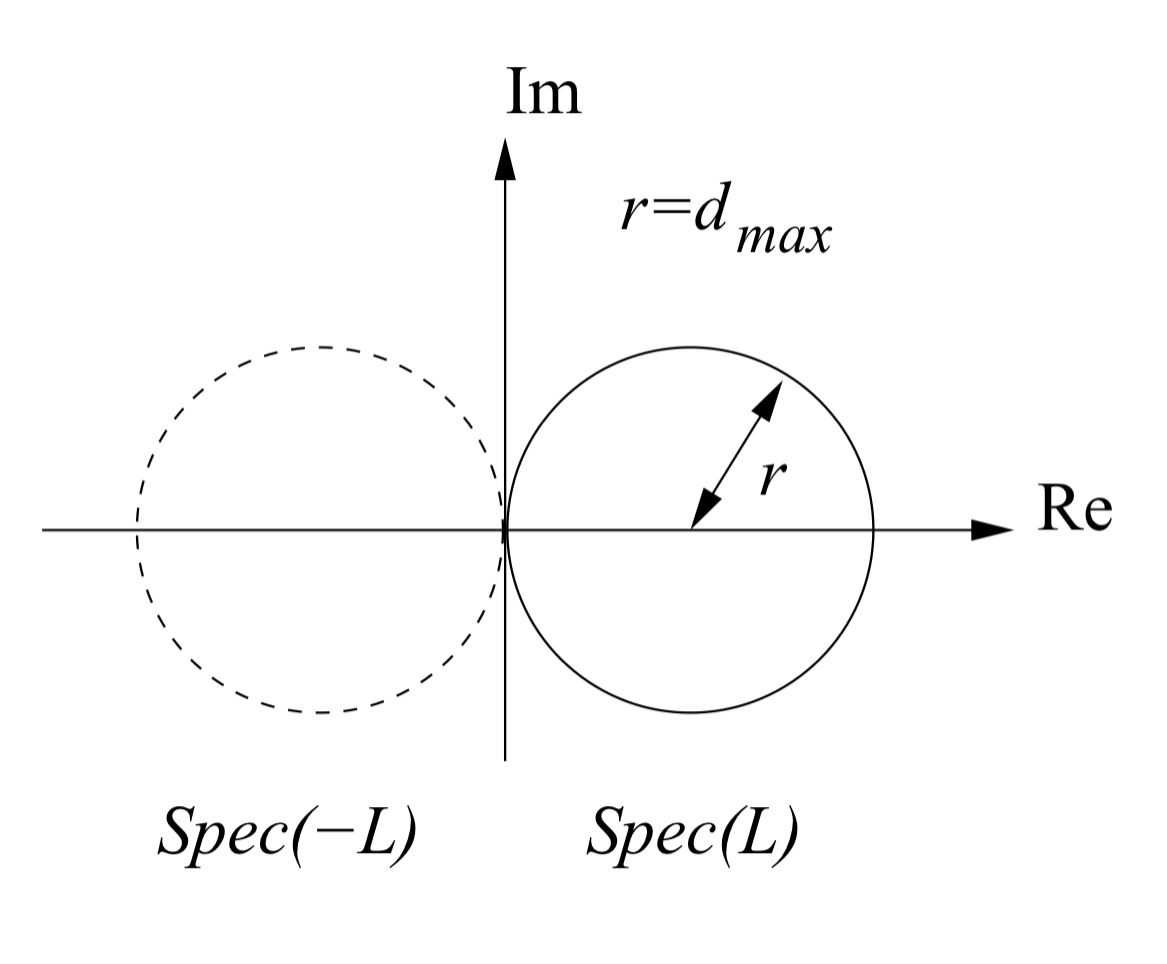
\includegraphics[width=8cm]{figures/Fig1-DiskTheorem.jpeg}
    \caption{圆盘定理应用在图拉普拉斯的效果演示}
    \label{DiskTheorem}
\end{figure}

\noindent \textbf{Proof.} 基于圆盘定理,所有$L=[l_{ij}]$的特征值都位于下面的$n$个圆盘的并集中
\begin{equation}
    D_i = \{ z\in \mathbb{C}: |z-l_{ii}| \le \sum_{j\in \mathcal{I},j\ne i}|l_{ij}| \}
    \tag{16}
    \label{16}
\end{equation}
如果$l_{ii} = \Delta_{ii}$那么
\begin{equation}
    \sum_{j\in \mathcal{I},j\ne i}|l_{ij}|=\deg_{out}(v_i) = \Delta_{ii}
    \notag
\end{equation}
因此,$D_i = \{ z\in \mathbb{C}:|z - \Delta_{ii}| \le \Delta_{ii}\}$。
另一方面,所有的$n$个圆盘被包含在一个最大的圆盘$D(G)$中,此圆盘半径为$d_{max}(G)$。
明显的,所有关于$-L$的特征值都位于$D(G)$关于虚轴镜像对阵的圆盘$D^\prime(G)=\{ z\in \mathbb{C}: |z+d_{max}(G)|\le d_{max}(G)\}$中。

以下是一个关于有向网络协议(\ref{A1})直接推论和首次收敛证明。

\noindent \textbf{Corollary 1.} 考虑到网络中的所有节点利用协议(\ref{A1})进行整合$\dot{x}_i = u_i$。
假设图$G$是强连接图。
那么,协议(\ref{A1})解决全局渐进一致性问题。

\noindent \textbf{Proof.} 由于$G$是强连接图,$\text{rank}(L)=n-1$并且$L$有一个为0的特征值。
基于定理2(Theorem 2),$-L$余下的特征值有负实部,并且因此线性系统(\ref{6})是稳定的。
另一方面,任何系统(\ref{6})的平衡状态$x^*$都是一个$L$关于$\lambda=0$的右特征向量。
由于特征空间是与0特征值有联系的1维特征向量,这里存在一个$\alpha\in \mathbb{R}$使得$x^*=\alpha\mathbf{1}$,即对于所有的$i$都有$x^*=\alpha$。

谨记推论1(Corollary 1)不能保证所有节点的决策值$\alpha$是否等于$\text{Ave}(x(0))$。
换句话说,推论1(Corollary 1)不一定能解决平均一致性问题。


\section{A Counterexample for Average-Consensus}
在推论1(Corollary 1)协议中,所有节点的每个决策值$\alpha$等于$\text{Ave}(x(0))$的充分条件是$\sum_{i=1}^{n}u_i \equiv 0$。
如果图$G$是无向图(即$a_{ij}=a_{ji} > 0,\forall i,j: a_{ij}\ne 0$),自动的情况$\sum_{i=1}^{n}u_i=0$,$\forall x$和$\text{Ave}(x(t))$是不变的量,参考文献[20]。
然而,这个性质并不适用于一般有向图。

一个简单的反例就是图(\ref{2})表示的3阶$n=3$强连接图,其中权重在\{0,1\}中,向量和边的集合如下所示:
\begin{equation}
    \mathcal{V} = \{1, 2, 3 \},\quad \mathcal{E}=\{12, 23, 31, 13\}.
    \notag
\end{equation}
\begin{figure}[htbp]
    \centering
    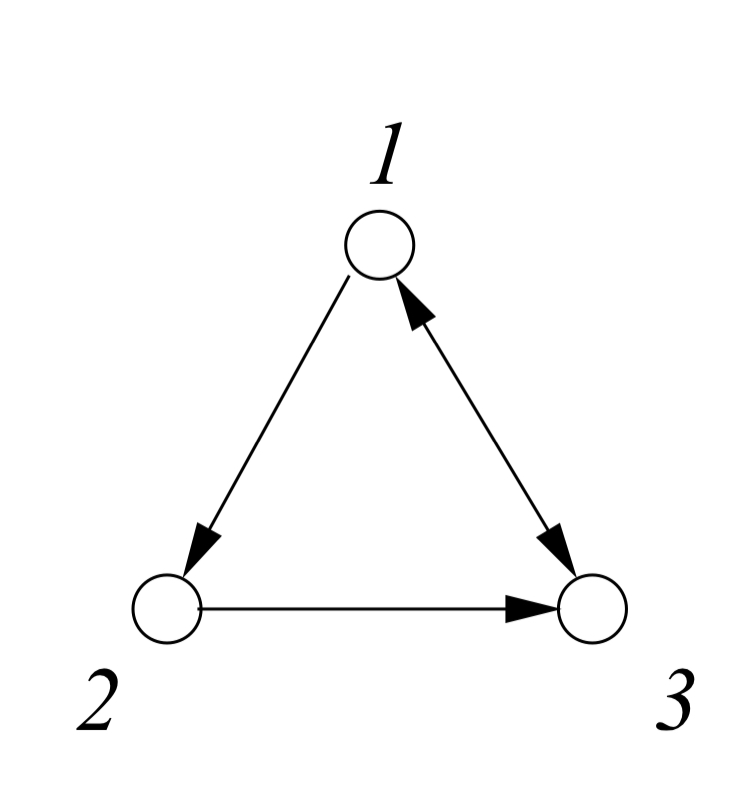
\includegraphics[width=4cm]{figures/Fig2-ConnectedDigraph.jpeg}
    \label{ConnectedDigraph}
    \caption{一个不能使用协议(\ref{A1})解决平均一致性问题的3阶连通图}
\end{figure}

对于图$G=(\mathcal{V}, \mathcal{E})$,$\sum_{i=1}^{3}u_i = x_3 - x_1$。
因此,如果节点1和3不一致,那么属性$\sum_{i=1}^{3}u_i = 0$不是对于所有的$x$都成立。
另一方面,读者可以在本例中来验证这一点
\begin{equation}
    L = \left[
    \begin{matrix}
        2 & -1 & -1 \\
        0 & 1 & -1 \\
        -1 & 0 & 1 
    \end{matrix}
    \right]
    \notag
\end{equation}

{\color{userColor}
\begin{equation}
    D = \left[
    \begin{matrix}
        2 & 0 & 0 \\
        0 & 1 & 0 \\
        0 & 0 & 1 
    \end{matrix}
    \right],
    A = \left[
    \begin{matrix}
        0 & 1 & 1 \\
        0 & 0 & 1 \\
        1 & 0 & 0 
    \end{matrix}
    \right],
    L = D - A
    \notag
\end{equation}
}

并且$x^*_i = [x_1(0) + x_2(0) + 2x_3(0)]/4$(此公式基于Theorem 3)。
这个决策值在所有$x_i(0)$的凸包中是显而易见的,但是当且仅当$x_1(0) + x_2(0) \ne 2x_3(0)$时,决策值不等于$\text{Ave}(x(0))$。
结果就是,对于所有初始条件满足$x_1(0) + x_2(0) \ne 2x_3(0)$,协议(\ref{A1})并不能解决平均一致性问题,但所有的节点仍能达到一致。
这促使我们描述所有的图的类,来解决平均一致性问题。

在提出我们第一次的主要结果之前,我们需要提供一个指数矩阵如$e^{(-Lt)}$形式的极限理论。
这是因为系统(\ref{6})的解决办法是通过以下公式给出
\begin{equation}
    x(t) = exp(-Lt)x(0)
    \tag{17}
    \label{17}
\end{equation}
并且通过对$exp(-Lt)$的显示计算,我们可以获得达到一致性的总图节点的决策值。
在非负矩阵理论中,接下来的定理与著名的极限定理关系密切,即Perron-Frobenius定理(Perron-Frobenius Theorem),参考文献[12]{\color[gray]{0.5}(R. A. Horn and C. R. Johnson. Matrix Analysis. Cambridge University Press, 1987)}。

\noindent \textbf{Notation.} 参考文献[12]的注解,我们记$M_{m,n}$为$m\times n$的实矩阵,$M_n$为$n \times n$的方阵。
进一步,通过这篇文章,关于$\lambda_1 = 0$的拉普拉斯矩阵$L$的右特征向量和左特征向量分别用$w_r$和$w_l$表示。

\noindent \textbf{Theorem 3.} 假设$G$是一个强连通图,拉普拉斯算子$L$满足$Lw_r=0$,$w_l^TL = 0$,$w_l^Tw_r=1$。
\begin{equation}
    R = \lim_{t\rightarrow +\infty} exp(-Lt) = w_r w_l^T \in M_n
    \tag{18}
    \label{18}
\end{equation}
\begin{equation}
    {\color{userColor} \text{R = t趋于无穷时-Lt关于e指数值极限 = 右特征向量 * 左特征向量}}
    \notag
\end{equation}

\noindent \textbf{Proof.} 令$A=-L$,$J$为$A$的约当形,即$A=SJS^{-1}$。
我们有$exp(At) = S\ exp(Jt)\ S^{-1}$当$s\rightarrow +\infty$,$exp(Jt)$收敛至一个具有单一非零元素$q_{11}=1$的矩阵$Q=[q_{ij}]$。
对角矩阵$exp(Jt)$的其他块会变成0,由于对于所有的$k\ge2$,都有$Re(\lambda_k(A))<0$,这里$\lambda_k(A)$是矩阵$A$的第$k$个最大的特征值$|A|$。
注意$R=SQS^{-1}$。
由于$AS=SJ$,$S$的第一列为$w_r$。
相似的,$S^{-1}A = JS^{-1}$,这也意味着$S^{-1}$的第一行是$w_l^T$。
由于$S^{-1}S=T$,$w_l$满足如性质所述的$w_l^Tw_r=1$。
直接的计算显示$R=w_rw_l^T\in M_n$。


\section{Networks with Fixed or Switching Topology}
这部分,我们提出了三种主要的结论:i)描述了所有使用协议(\ref{A1})解决平均一致性问题的连接图。
ii)协议(\ref{A1})的性能和图的费德勒特征值(即代数连接)之间的联系。
iii)在切换拓扑下的连接失败/生成的鲁棒一致性问题。

\subsection{Balanced Graphs and Average-Consensus on Digraphs}
下述的图类表明了在解决一致性问题的分析:

\noindent \textbf{Definition 1.} (平衡图)我们认为当且仅当图$G=(\mathcal{V}, \mathcal{E}, \mathcal{A})$的节点$v_i$的入度(in-degree)等于出度(out-degree)时,节点是平衡的,即$\deg_{out}(v_i)=\deg_{in}(v_i)$。
当图$G=(\mathcal{V}, \mathcal{E}, \mathcal{A})$的所有节点都是平衡时,图是平衡图,即$\sum_{j}a_{ij} = \sum_{j}a_{ji}, \forall i$。

\noindent \textbf{Example 1.} 任意的无向图都是平衡的。
进一步说,图\ref{3}展示的图都是平衡的{\color{userColor}(总的出度=总的入度,不是每一个节点都需要相等)}。
\begin{figure}[htbp]
    \centering
    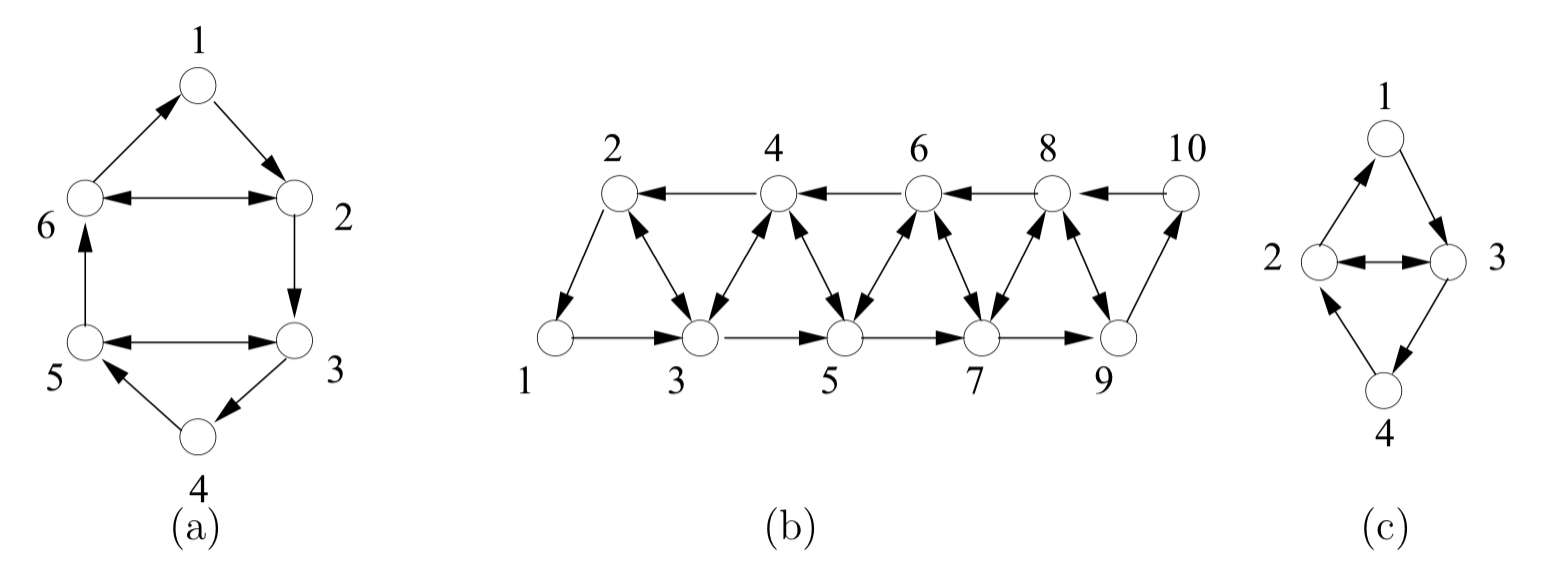
\includegraphics[width=12cm]{figures/Fig3-BalancedGraphs.jpeg}
    \label{BalancedGraphs}
    \caption{平衡图的三个例子}
\end{figure}

接下来是我们的第一个主要结论:

\noindent \textbf{Theorem 4.} 考虑一个有向信息流网络$G=(\mathcal{V}, \mathcal{E}, \mathcal{A})$的整合,网络是强连通的。
那么,当且仅当图$G$是平衡图时,协议(\ref{A1})全局渐进的解决了平均一致性问题。

\noindent \textbf{Proof.} 证明参考如下定理5和定理6。

\noindent {\em Remark} 5. 根据定理4,如果图不是平衡图,那么协议(\ref{A1})没有办法解决平均一致性问题。
此断言与图\ref{ConnectedDigraph}给出的反例是一致的。

\noindent \textbf{Theorem 5.} 考虑一个整合智能体网络图$G=(\mathcal{V}, \mathcal{E}, \mathcal{A})$是强连接的。
那么,当且仅当$\mathbf{1}^TL=0$时,协议(\ref{A1})全局渐进的解决了平均一致性问题。

\noindent \textbf{Proof.} 参考定理3,结合$w_r = \frac{1}{\sqrt{n}}\mathbf{1}$我们可以得到
\begin{equation}
    x^* = \lim_{t\rightarrow +\infty}x(t) = Rx_0 = w_r(w_L^T x_0) = \frac{1}{\sqrt{n}}(w_l^Tx_0)\mathbf{1}
    \notag
\end{equation}
这表明协议1全局指数解决了每一个节点关于决策值$\frac{1}{\sqrt{n}}(w_l^Tx_0)$的一致性问题。
如果这个决策值等于$Ave(x_0), \forall x_0 \in \mathbb{R}^n$,那么必要的$\frac{1}{\sqrt{n}}w_l = \frac{1}{\sqrt{n}}$,即$w_l= w_r=\frac{1}{\sqrt{n}}\mathbf{1}$。
这表明$\mathbf{1}$是关于$L$的左特征向量。
为了证明一致性,假设$\mathbf{1}^TL=0$。
我们令$w_r=\frac{1}{\sqrt{n}}\mathbf{1}$,$w_l=\beta\mathbf{1},\beta\in\mathbb{R},\beta\ne0$。
根据条件$w_l^Tw_r=1$,我们得到$\beta=\frac{1}{\sqrt{n}}$和$w_l=\frac{1}{\sqrt{n}}\mathbf{1}$。
这意味着每一个节点的决策值是$\frac{1}{\sqrt{n}}(w_l^Tx_0)=\frac{1}{n}\mathbf{1}^Tx_0=Ave(x_0)$。

\noindent \textbf{Corollary 2.} 假设定理5中的所有条件成立。
假设$L$有一个关于特征值$\lambda=0$的左特征向量$\gamma = (\gamma_1, \dots, \gamma_n)^T$,这是一个属于$\mathbb{R}$的非负向量(即向量元素非负)且满足$\sum_i\gamma_i>0$。
那么,达到一致的群组决策值就是:
\begin{equation}
    \alpha = \frac{\sum_i \gamma_ix_i(0)}{\sum_i\gamma_i}
    \tag{19}
    \label{19}
\end{equation}
即决策值是在节点初始值的凸包中。

\noindent \textbf{Proof.} 
我们有$\gamma^TL=0$并且因此$\gamma^Tu\equiv0$(因为$u=-Lx$)的集合。
因此,$\beta=\gamma^Tx$是一个不变的量。
假如,图$G$是不平衡的。
那么,一致性仍是渐进达到的。
定义$\alpha$是所有节点达到一致后的决策值。
我们有$\gamma^Tx^*=\gamma^Tx(0)$由于不变的$\gamma^Tx(0)$。
但是$x^*=\alpha\mathbf{1}$,因此我们得到
\begin{equation}
    (\sum_i\gamma_i)\alpha = \gamma^Tx(0)
    \notag
\end{equation}

接下来的结果显示了,如果其中一个智能体使用了一个相当小的更新速率(或step-size),即$\gamma_{i^*}\gg\gamma_i$对所有的$i\ne i^*$。
那么,所有节点的决策值收敛到$x_{i^*}$。
换句话说,智能体$i^*$在领导者跟随(leader-follower)结果类型中扮演领导者的角色。

\noindent \textbf{Corollary 3.} (多比例积分)考虑一个多比例积分网络,其节点动态如下:
\begin{equation}
    \gamma_i \dot{x}_i=u_i,\quad \gamma_i>0,\forall i \in \mathcal{I}
    \tag{20}
    \label{20}
\end{equation}
假设每一个节点满足协议(\ref{A1})。
那么,达到一致的群组决策值就是:
\begin{equation}
    \alpha = \frac{\sum_i \gamma_ix_i(0)}{\sum_i\gamma_i}
    \tag{21}
    \label{21}
\end{equation}

\noindent \textbf{Proof.} 网络根据下式动态变化:
\begin{equation}
    D\dot{x} = -Lx
    \notag
\end{equation}
这里,$D=diag(\gamma)$是关于第$i$个对角元素对角矩阵,对角元素满足$\gamma_i>0$。
后边的公式可以写成为:
\begin{equation}
    \dot{x} = -\tilde{L}x
    \notag
\end{equation}
这里,$\tilde{L} = D^{-1}L = diag(\frac{1}{\gamma_1},\dots,\frac{1}{\gamma_n})L$是图$\tilde{G}$和邻接矩阵$\tilde{A}=D^{-1}\mathcal{A}$(即从节点$i$离开的边的权重被$\gamma_i$分割)的拉普拉斯矩阵。
清晰的,$\gamma$是一个正元素向量,它是$\tilde{L}$的左特征向量,并且基于推论2的决策值是位于被$x_i(0)^\prime s$平均权重中被$\gamma$。

\noindent {\em Remark} 6. Jadbabaie等人讨论了关于公式(\ref{20})和协议(\ref{A1})的一阶Euler渐进(Euler approximation)离散时间模型和姿态位置协议,推论3中$\gamma_i=deg_{out}(v_i)+1$的特殊选择。
在文献[6],拉普拉斯矩阵被定义为$I-D\mathcal{A}$,在本文中这等价于一个$\gamma_i=deg_{out}(v_i)\ge 0$多比例整合网络。
$D$的奇异性由$\gamma_i=deg_{out}(v_i)$的选择决定,这在文献[13]中通过增加合适的正常量(即1)到$deg_{out}(v_i)$中来避免。

\noindent \textbf{Theorem 6.} 定义一个具有邻接矩阵$\mathcal{A}=[a_{ij}]$的图$G=(\mathcal{V}, \mathcal{E}, \mathcal{A})$。
那么,下列所有的条件都是等价的:

i)图$G$是平衡的;

ii)$w_l = \mathbf{1}$是图$G$拉普拉斯算子相对于0特征值的左特征向量,即$\mathbf{1}^TL = 0$。

iii)有$\sum_{i=1}^n u_i = 0$,对于所有的$\forall x \in \mathbb{R}$,$u_i = \sum_{j\in N_i}a_{ij}(x_j - x_i)$。

\noindent \textbf{Proof.} 我们展示了i)$\Leftrightarrow$ii)和ii)$\Leftrightarrow$iii)。

对于i)$\Leftrightarrow$ii)的证明:
我们有$\Delta_{ii} = deg_{out}(v_i)$和$deg_{in}(v_i)=\sum_{j,j\ne i}a_{ji}$,因此矩阵$L$第$i$列的和等于
\begin{equation}
    \sum_il_{ji} = \sum_{i,j\ne i}l_{ji}+l_{ii} = -deg_{in}(v_i) + deg_{out}(v_i) = 0 \Leftrightarrow \text{图}G\text{的节点}i\text{是平衡的}
    \notag
\end{equation}
注意到矩阵$L$第$i$列的和等于向量$\mathbf{1}^TL$的第$i$个行元素,可以推断如果图$G$的所有节点是平衡,那么$\mathbf{1}^TL$,即图$G$是不平衡的。

对于ii)$\Leftrightarrow$iii)的证明:
由于$u=-Lx$,($\sum_iu_i=0,\forall x$)$\Leftrightarrow$ ($\mathbf{1}^Tu=-(\mathbf{1}^TL)x=0, \forall x$)$\Leftrightarrow$ $\mathbf{1}^TL=0$。

\noindent {\em Remark} 7. 注意在定理6中,图$G$不需要连通。

\subsection{Performance of Group Agreement and Mirror Graphs}
在这部分,我们讨论协议(\ref{A1})平衡图的一些问题。
定理6的一个重要的结果就是对于平衡信息流网络而言,$\alpha = Ave(x)$是一个不变的量。
对于任意的有向图,并不是确定正确的。
$Ave(x)$的不变性允许其根据以下方程进行$x$的分解:
\begin{equation}
    x = \alpha \mathbf{1} + \delta
    \tag{22}
    \label{22}
\end{equation}
这里,$\alpha = Ave(x)$,$\delta\in \mathbb{R}^n$且满足$\sum_i\delta_i=0$。
我们引用$\delta$作为(群组)非一致向量。
向量$\delta$与$\mathbf{1}$正交,且属于一个$(n-1)$-维子空间,此子空间叫做强连通图$G$的拉普拉斯矩阵$L$的非一致特征空间。
此外,$\delta$根据下边给出的动态非一致(群组)公式变化
\begin{equation}
    \dot{\delta} = -L\delta
    \tag{23}
    \label{23}
\end{equation}

定义图$G$的拉普拉斯非一致函数为:
\begin{equation}
    \Phi_G(x) = x^T Lx
    \tag{24}
    \label{24}
\end{equation}
此时$L=\mathcal{L}(G)$。
对于图,$\Phi_G(x)$可以是负定的(例如,两个节点和一个边12的图拉普拉斯矩阵是非半正定的)。

这也证明平衡图的一个有效性质是,他们的拉普拉斯算子非一致函数是半正定的。
另外,对于任意的平衡图$G$,都存在一个具有相同拉普拉斯非一致函数的无向图$G$。
接下来,我们正式定义这个感应无向图。

\noindent \textbf{Definition 2.} (镜像图/操作)定义加权有向图$G=(\mathcal{V}, \mathcal{E}, \mathcal{A})$。
定义$\tilde{\mathcal{E}}$是图$G$的反转边(reverse edges)的一部分,图$G$通过反转$\mathcal{E}$中所有成对节点的顺序得到。
图$G$的镜像(mirror)定义为$\hat{G}=\mathcal{M}(G)$,它是一个形式为$\hat{G}=(\mathcal{V}, \hat{\mathcal{E}}, \hat{\mathcal{A}})$的无向图,具有和$G$一样的节点,边$\hat{\mathcal{E}}=\mathcal{E}\cup \tilde{\mathcal{E}}$,和渐进邻接矩阵$\hat{\mathcal{A}}=[\hat{a}_{ij}]$元素为
\begin{equation}
    \hat{a}_{ij}=\hat{a}_{ji}=\frac{a_{ij}+a_{ji}}{2}\ge 0
    \tag{25}
    \label{25}
\end{equation}

接下来的结果展示了关于$\mathcal{L}$和在加权邻接矩阵$\mathcal{A}$进行交换时符号的操作。

\noindent \textbf{Theorem 7.} 定义$G$是一个具有邻接矩阵$\mathcal{A}=adj(G)$和拉普拉斯矩阵$L=\mathcal{L}(G)$的图。
那么$L_s = Sym(L) = (L+L^T)/2$是一个关于$\hat{G}=\mathcal{M}(G)$的可用拉普拉斯矩阵,此时$G$是平衡图,即下述图转换当且仅当$G$是平衡的
\begin{equation}
    \begin{aligned}
                    &G \xrightarrow{adj}         &\mathcal{A} \xrightarrow{\mathcal{L}}          &L \\
        \mathcal{M} &\downarrow \quad\quad Sym   &\downarrow  Sym                      &\downarrow \\
                    &\hat{G} \xrightarrow[adj]{} &\hat{\mathcal{A}} \xrightarrow[\mathcal{L}]{}  &\hat{L} 
    \end{aligned}
    \tag{26}
    \label{26}
\end{equation}
此外,如果$G$是平衡图,那么$G$的拉普拉斯非一致函数和$\hat{G}$是相等的。

\noindent\textbf{Proof.} 我们知道$G$是平衡的当且仅当$\textbf{1}^TL=0$。
由于$L\textbf{1}=0$,我们有$\mathbf{1}^TL=0$ $\Leftrightarrow$ $\frac{1}{2}(L+L^T)\mathbf{1}=0$。
因此$G$是平衡的当且仅当$L_s$有一个关于$\lambda=0$右特征向量$\mathbf{1}$,即$L_s$是一个可用拉普拉斯矩阵。
现在,我们证明$L_s=\mathcal{L}(\hat{G})$。为了证明,我们计算$\hat{\Delta}$的元素,可以得到:
\begin{equation}
    \hat{\Delta}_{ii}=\sum_j \frac{a_{ij}+a_{ji}}{2}=\frac{1}{2}(deg_{out}(v_i)+deg_{in}(v_i))=deg_{out}(v_i)=\Delta_{ii}
    \notag
\end{equation}
因此,$\hat{\Delta}=\Delta$。
另一方面,我们有
\begin{equation}
    L_s = \frac{1}{2}(L+L^T) = \Delta-\frac{A+A^T}{2}=\hat{\Delta}-\hat{A}=\hat{L}=\mathcal{L}(\hat{G})
    \notag
\end{equation}
最后一部分来源于$\hat{L}$等于$L$的渐进部分,且$x^T(L-L^T)x\equiv0$。

\noindent\textbf{Notation.} 为了简化符号,在代数图论部分,$\lambda_k(G)$用来表示$\lambda_k(\mathcal{L}(G))$。

现在,我们准备展示对协议(\ref{A1})关于群组达到一致性速度的研究结果。

\noindent\textbf{Theorem 8.} (一致性的性能)考虑带有有向信息流$G$且是平衡和强连通的积分器网络。
那么,给出协议(\ref{A1}),下述状态满足:

i)群组的非一致向量$\delta$是非一致变化在公式(\ref{23})全局渐进消失的答案,消失速度等于$\kappa=\lambda_2(\hat{G})$(或图$G$镜像的费德勒特征值),即
\begin{equation}
    \tag{27}
    \label{27}
    ||\delta(t)||\le ||\delta(0)||exp(-kt)
\end{equation}

ii)下述的流畅的,正向无限制,前者函数
\begin{equation}
    \tag{28}
    \label{28}
    V(\delta) = \frac{1}{2}||\delta||^2
\end{equation}
是一个可用的非一致动态变化的李雅普诺夫函数。

\noindent\textbf{Proof.} 我们有
\begin{equation}
    \tag{29}
    \label{29}
    \dot{V} = -\delta^TL\delta = -\delta^TL_s\delta = -\delta^T\hat{L}\delta \le -\lambda_2(\hat{G})||\delta||^2 = -2\kappa V(\delta) < 0, \forall \delta \ne 0
\end{equation}
这证明$V(\delta)$是一个可用的关于群组动态非一致的李雅普诺夫函数。
此外,$\delta(t)$全局指数消失速度为$\kappa$由$t\rightarrow +\infty ..$。
事实上$L_s = \hat{L}$是一个关于无向图(即$G$的镜像)的可用拉普拉斯矩阵,来源定理7且不相等
\begin{equation}
    \tag{30}
    \label{30}
    \delta^T \hat{L} \delta \ge \lambda_2(\hat{G})||\delta||^2,\quad \forall\delta:\mathbf{1}^T\delta=0
\end{equation}
这来源于公式(\ref{14})。

众所周知的现象关于无向图的费德勒特征值,对于密集图$\lambda_2$是相当大的,而对于稀疏图$\lambda_2$是相当小的[11](这是为什么$\lambda_2$被叫做代数连通度)。
根据这个现象,根据定理8,可以推断具备密集内连接的网络比一个连接但稀疏的网络能更快的解决一致性问题。
这和关于关于群组一致性的常识是一致的。
特殊的,能创造一个$n$节点平衡图长度为$n$的图解决了一致性问题。
然而,这是一种很慢的解决一致性问题的方式。


\subsection{Consensus in Networks with Switching Topology}
考虑一个具有移动智能体的网络,之间互相沟通并且需要一致到一个感兴趣的目标或表现同步。
由于网络节点一直在移动,不难想象,由于两个智能体之间存在障碍物,通信连接很容易丢失。
由于智能体进入了其他智能体的有效检测范围,那么就会发生相邻智能体之间出现新连接的对立情况。
换句话说,在用图$G$表示的有限信息流网络中,图$G$的某些边缘会增加或移除。
在这里,我们致力于发现探索网络具有切换拓扑的情况,无论是否能够达到一致性。

考虑一个具有连续状态和离散状态的混合系统,这属于有限集合图$G$
\begin{equation}
    \Gamma_n = \{ G: G\ \text{is a digraph of order}\ n\ \text{that is}\ strongly\ connected\ \text{and}\ balanced \}
    \notag
\end{equation}
可以被分析表示成如下形式:
\begin{equation}
    \Gamma_n = \{ G=(\mathcal{V}, \mathcal{E}, \mathcal{A}): \text{rank}(\mathcal{L}(G)) =n-1, \mathbf{1}^T\mathcal{L}(G) = 0\}
    \tag{31}
    \label{31}
\end{equation}

给出节点的动态协议,那么系统的连续状态根据如下动态进行演变:
\begin{equation}
    \dot{x}(t) = -\mathcal{L}(G_k)x(t),\quad k=s(t), G_k\in \Gamma_n
    \tag{32}
    \label{32}
\end{equation}
这里,$s(t): \mathbb{R}_{\ge 0}\rightarrow \mathcal{I}_{\Gamma_n}$是切换信号(switching signal),并且$\mathcal{I}_{\Gamma_n}\subset \mathbb{N}$是相对于$\Gamma_n$中元素的索引集合。
清晰的,$\Gamma_n$是一个有限集合,因为它不是一个没有边缘的图,而是一个具有$n(n-1)$个边的完整图。
解决具有切换拓扑的移动网络的一致性问题的关键是,公式(\ref{28})提到的李雅普诺夫函数的基本性质和平衡图的性质。
注意函数$V(\delta)=\frac{1}{2}||\delta||^2$并不依赖$G$或$L=\mathcal{L}(G)$。
$V(\delta)$的这个性质使它成为切换拓扑系统(\ref{32})的李雅普诺夫函数稳定性分析的合适候选。

\noindent \textbf{Theorem 9.} 对于任意的切换信号$s(\cdot)$,切换系统(\ref{32})的解决方法是全局渐进收敛到$Ave(x(0))$(即完成平均一致性)。
此外,下述的平滑,正定,合适函数
\begin{equation}
    V(\delta) = \frac{1}{2}||\delta||^2
    \label{33}
    \tag{33}
\end{equation}
是一个下面给出的关于动态非一致性协议普遍可用的李雅普诺夫方程
\begin{equation}
    \dot{\delta}(t) = -\mathcal{L}(G_k)\delta(t),\quad k=s(t),G_k\in \Gamma_n.
    \tag{34}
    \label{34}
\end{equation}

进一步的,非一致性向量$\delta$随着关于下述的最小速率呈指数级消失
\begin{equation}
    \kappa^* = \min_{G\in \Gamma_n} \lambda^2(\mathcal{L}(\hat{G})).
    \tag{35}
    \label{35}
\end{equation}
也就是说,$||\delta(t)||\le ||\delta(0)||exp(-\kappa^*t)$。

\noindent \textbf{Proof.}
根据$G_k$是平衡图的事实,对于所有的$k$和$u=-\mathcal{L}(G_k)x$,我们有$\mathbf{1}^Tu=-(\mathbf{1}^T\mathcal{L}(G_k))x\equiv0$。
因此,$\alpha=Ave(x)$是一个不变量,允许分解$x$为$x=\alpha \mathbf{1}+\delta$。
因此,由公式(\ref{32})引起的非一致切换系统变为公式(\ref{34})的形式。
计算$\dot{V}$,我们得到
\begin{equation}
    \tag{36}
    \label{36}
    \dot{V} = \delta^T\mathcal{L}(G_k)\delta = -\delta^T\mathcal{L}(\hat{G}_k)\delta \le -\lambda_2(\mathcal{L}(\hat{G}_k))||\delta||^2 \le -\kappa^*||\delta||^2 = -2\kappa^*V(\delta)<0,\forall \delta \ne 0
\end{equation}
这保证了$V(\delta)$是一个关于非一致切换系统(\ref{34})的普通李雅普诺夫函数。
此外,我们有
\begin{equation}
    \notag
    V(\delta(t)) \le V(\delta(0))exp(-2\kappa^*t) \Rightarrow ||\delta(t)|| \le ||\delta(0)||exp(-\kappa^*t)
\end{equation}
并且非一致性向量$\delta(t)$全局指数消失速度为$\kappa^* > 0$为$t\rightarrow +\infty$。
最后,公式(\ref{35})的最小化总是存在并且是可以得到的,因为$\Gamma_n$是一个有限集合。


\section{Networks with Communication Time-Delays}
考虑固定拓扑$G=(\mathcal{V}, \mathcal{E}, \mathcal{A})$连续时间网络,其节点$i$的状态经过一个时滞$\tau > 0$的通信通道(或连接)达到节点$j$。
关于连接$ij$的转移函数表示如下:
\begin{equation}
    h_{ij}(s) = e^{-\tau_{ij}s}
    \notag
\end{equation}
应用线性时滞协议(\ref{A2}),网络动态变化可写作:
\begin{equation}
    \dot{x}_i(t) = \sum_{j\in N_i} a_{ij} [x_j(t-\tau_{ij}) - x_i(t-\tau_{ij})].
    \tag{37}
    \label{37}
\end{equation}
通过对公式(\ref{37})两边进行拉氏变换,我们得到
\begin{equation}
    sX_i(s) - x_i(0) = \sum_{j\in N_i} a_{ij} h_{ij}(s) (X_j(s) - X_i(s))
    \tag{38}
    \label{38}
\end{equation}
这里$X_i(s)$表示所有$i\in \mathcal{I}$中$x_i(t)$的拉氏变换。
公式的最后一部分可以写作如下紧凑形式:
\begin{equation}
    X(s) = (s+L(s))^{-1}x(0)
    \tag{39}
    \label{39}
\end{equation}
这里$L(x)$是图关于邻接矩阵$\mathcal{A}(s) = [a_{ij}h_{ij}(s)]$的拉普拉斯矩阵。
总的来说,任何关于通道$ij$的过滤效果都可以合并成连接转换函数$h_{ij}(s)$。
关于通信时滞智能体网络的协议(\ref{A2})收敛性分析减小为一个多输入多输出系统(MIMO)转移函数的稳定性分析
\begin{equation}
    G(s) = (sI+L(s))^{-1}.
    \notag
\end{equation}

为了得到图拉普拉斯算子和一致性协议(\ref{A2})收敛性质之间进一步关键点,我们聚焦在最简单的可能情况,这里所有通道的时滞都等于一个无向固定拓扑图$G$网络中的$\tau > 0$。
立即推,其遵循$\sum_i u_i \equiv 0$并且因此$\alpha = Ave(x(t))$是一个不变的量。
另外,我们有
\begin{equation}
    L(s) = e^{-\tau s}L
    \notag
\end{equation}
这里$L=\mathcal{L}(G)$。
这是我们关于通信时滞网络(\ref{20})一致性协议的主要研究成果。

\noindent \textbf{Theorem 10.} 考虑一个带有相等通信时滞$\tau > 0$的智能体网络。
假设网络信息流$G$是无向且连通的。
那么,当且仅当以下两个等价情况任何一个满足时,带有$\tau_{ij} = \tau$的协议(\ref{A2})能全局渐进解决平均一致性问题:

i)$\tau \in (0, \tau^*)\ \text{with}\ \tau^*=\frac{\pi}{2\lambda_n}, \lambda_n=\lambda_{max}(L)$.

ii)关于$\Gamma(s) = e^{-\tau s}/s$的奈奎斯特图(Nuquist plot)有在$-1/\lambda_k,\ \forall k > 1$附近的零包围。

此外,对于$\tau=\tau^*$,系统有关于频率$w=\lambda_n$的全局渐进稳定振荡解决方案。

\noindent \textbf{Proof.} 证明过程详见附录A.2。

基于定理10的i),可以推断网络的时滞可受理通道的上界是$\lambda_n$的相反部分,即信息流拉普拉斯矩阵的最大特征值。
根据盖尔圆定理,我们可以知道$\lambda_n\le 2d_{max}(G)$,这里$d_{max}(G)$是图$G$节点的最大出度。
因此,收敛性协议(\ref{A2})的一个充分条件是:
\begin{equation}
    \tau \le \frac{\pi}{4d_{max}(G)}
    \tag{40}
    \label{40}
\end{equation}
这也就意味着具有高出度节点的网络不能忍受相当高的沟通时滞。
另一方面,使$\tilde{\mathcal{A}}=k\mathcal{A}$,$k>0$是$\tilde{G}$的邻接矩阵。
定义$\tilde{L}=\mathcal{L}(\tilde{G})$,并且记$\lambda_n(\tilde{L}) = k\lambda_n(L)$。
因此,对于任意大小的延迟$\tau>0$,都存在一个足够小的$k>0$使得$\tau < \pi/(2k\lambda_n)$。
结果就是,通过调整图权重的大小,任意大小的时滞都能忍受。
权衡的是因子$1/k>0$协商速度。
换句话说,在一致性算法的鲁棒性和时滞收敛速度之间存在权衡。


\section{Max-Consensus and Leader Determination}
在这部分,我们讨论带有一个唯一的最大领导者(max-leader)网络的最大一致性问题,即节点$i^*=\arg\max_ix_i(0)$。
最大一致性问题描述如下。
每一个智能体都有下述离散模型
\begin{equation}
    \tag{41}
    \label{41}
    x_i(k+1)=max(x_i(k),u_i(k))
\end{equation}
且被称作最大智能体(max-agent)。
最大智能体的动态等价描述为一个非线性离散时间系统如下:
\begin{equation}
    \tag{42}
    \label{42}
    x_i(k+1) = \frac{1}{2}(x_i(k)+u_i(k)+|x_i(k)-u_i(k)|)
\end{equation}
图$G=(\mathcal{V},\mathcal{E})$所有节点的值必须反复收敛到最大领导者的值。
另外,分布式的每一个节点都必须决定其是否是最大领导者。
最大一致性问题的一个应用是决定群组中的领导者(或协调者)具备关于特别兴趣量(例如,序列号,花费,高度,等等)的优先级,其必须执行或协调任务。

我们使用下述协议来解决最大一致性问题:
\begin{equation}
    \tag{A4}
    \label{A4}
    u_i(k) = \max_{j\in N_i}x_j
\end{equation}

\noindent{\em Remark} 8. 表现上,最小一致性问题(min-consensus problem)能被最大一致性问题类似的定义和解决,这里不再讨论。

注意到最大智能体的值是非减的,即所有的$i\in\mathcal{I}$都有$x_i(k+1)\ge x_i(k)$。
为了保持追踪一个节点是否是最大领导者,我们使用一个叫做最大标记(max-flag)的布尔变量$f_i(k)\in\{0,1\}$来扩大每个节点的状态。
最大标记(max-flag)根据下述规则(或状态反馈)变化:
\begin{equation}
    \tag{43}
    \label{43}
    f_i(k+1) = K(f_i(k),x_i(k),u_i(k)):=
    \left\{
        \begin{matrix}
            f_i(k)\quad x_i(k+1)=x_i(k)\\
            \bar{f}_i(k) \quad x_i(k+1)>x_i(k)
        \end{matrix}
    \right.
\end{equation}
这里的bar操作是布尔变量无效。
最初的,所有的节点他们都是最大领导者,或所有的$i$都是$f_i(0)=1$。
如果即节点的值相比与最初的值增加了,那么它就意味着不再是最大领导者。

\noindent\textbf{Theorem 11.} 考虑一个最大智能体网络具有如下动态变化:
\begin{equation}
    \tag{44}
    \label{44}
    \left\{
        \begin{matrix}
            x_i(k+1) = \max(x_i(k),u_i(k))\\
            f_i(k+1) = K(f_i(k),x_i(k),u_i(k))
        \end{matrix}
    \right.
\end{equation}
这里映射$K:\{0,1\}\times \mathbb{R}\times\mathbb{R}\rightarrow\{0,1\}$定义在公式(\ref{43})。
假设$G=(\mathcal{V},\mathcal{E})$是一个强连通图。
那么,协议(\ref{A4})在有限次迭代$l\le n-1$中解决了最大一致性问题,即所有节点值收敛到最大领导者的值,最大标记的值而不是最大领导者的值收敛到0在$O(n)$时间。

\noindent\textbf{Proof.} 令$l$为连接每个节点到最大领导者的最短路径的最大长度。
由于图$G$是强连通的$l\le n-1$。
观察到最大领导者的值$\alpha=x_i(k)$在时间内保持不变,因为所有其他节点的值是小于最大领导者的值,公式(\ref{43}),$f_{i^*}(k)=f_{i^*}(0)=1$对所有的$k>0$。
类似于关于定理1的证明,使$J^{(k)}$表示一个关于最大领导者$i^*$的第$k$个邻居簇(关于$J^{(k)}$的定义,看附录中的公式(\ref{46})。
给出协议(\ref{A4}),很容易便可看到节点$i^*$的第$k$个邻居簇的所有节点变得等于$\alpha$,所有在$j^{(k)}\backslash {i^*}$中的节点最大标记在$k$此迭代后变为0。
另一方面,关于$l\le n-1$的定义,$J^{(l)}=\mathcal{I}$和结果在之后。


\section{Simulation Results}
\begin{figure}[htbp]
    \centering
    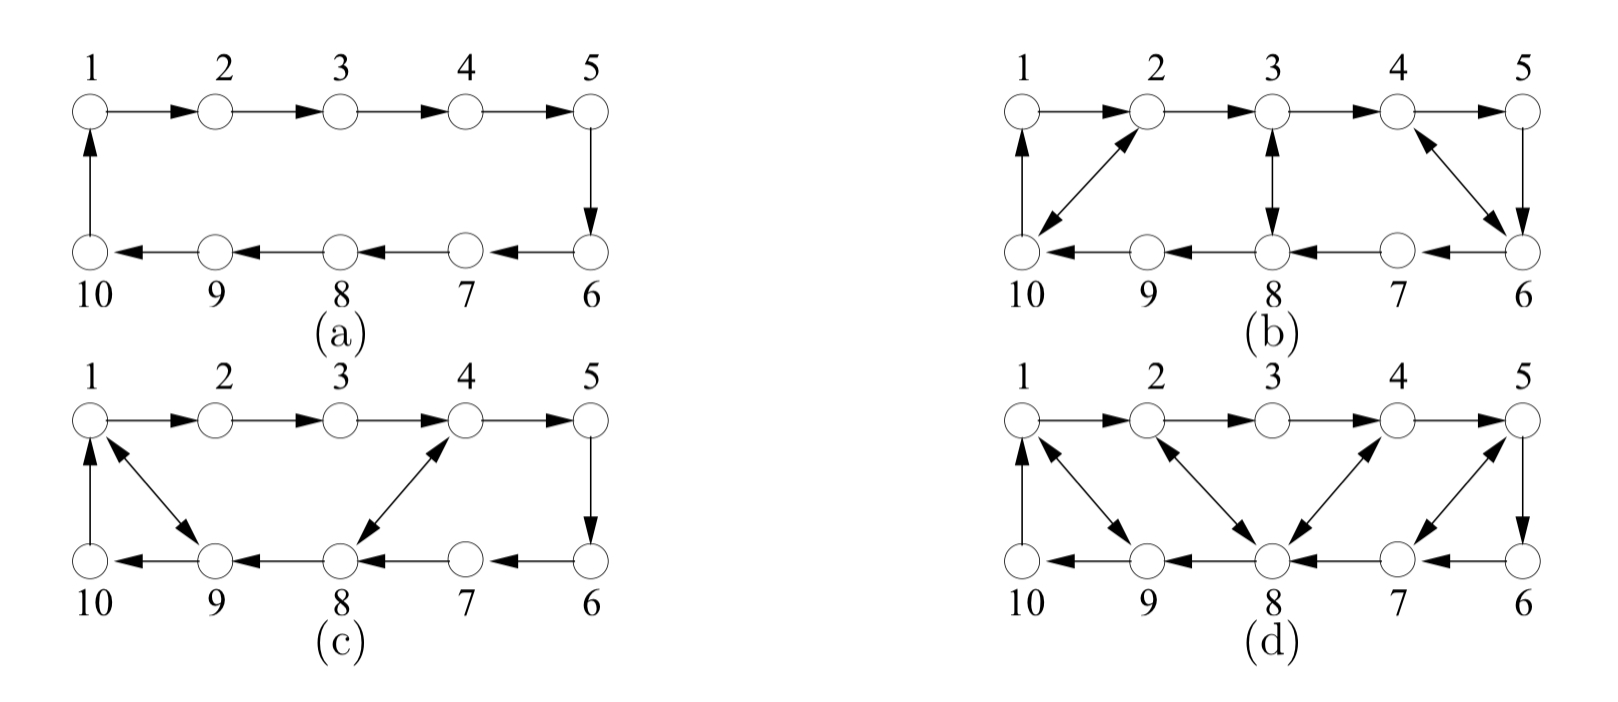
\includegraphics[width=12cm]{figures/Fig4-BalancedSC.jpeg}
    \label{Fig4}
    \caption{强连接的平衡图}
\end{figure}

图(4)展示了四个不同的网络,每个都有$n=10$个节点,这些网络都是强连接并且平衡的。
与所有边相关的权重大小都是1。
对于以下的节点初始值都满足$\text{Ave(x(0))} = 0$
\begin{equation}
    x(0) = (−10.2999, 0.2575, −4.4997, 3.6258, 3.0922, 9.0156, 3.5099, −2.6645, 2.4552, −4.4921)^T
    \notag
\end{equation}
我们已经绘制出状态轨迹,和关于这四个图的非一致函数$||\delta||^2$,如图(5)所示。
可以清楚的知道,随着图的边的数量的增加,代数连通度(或$\lambda^2$)增加,节点的轨迹稳定时间减小。
长度为$n=10$或$G_a$的有向周期,具有最大的过冲情况。
在所有的四种情况下,一致性都是逐渐达到的,并且性能随着函数$\lambda_2(\hat{G}_k)$而改善,其中$k\in \{a,b,c,d\}$。

\begin{figure}[htbp]
    \centering
    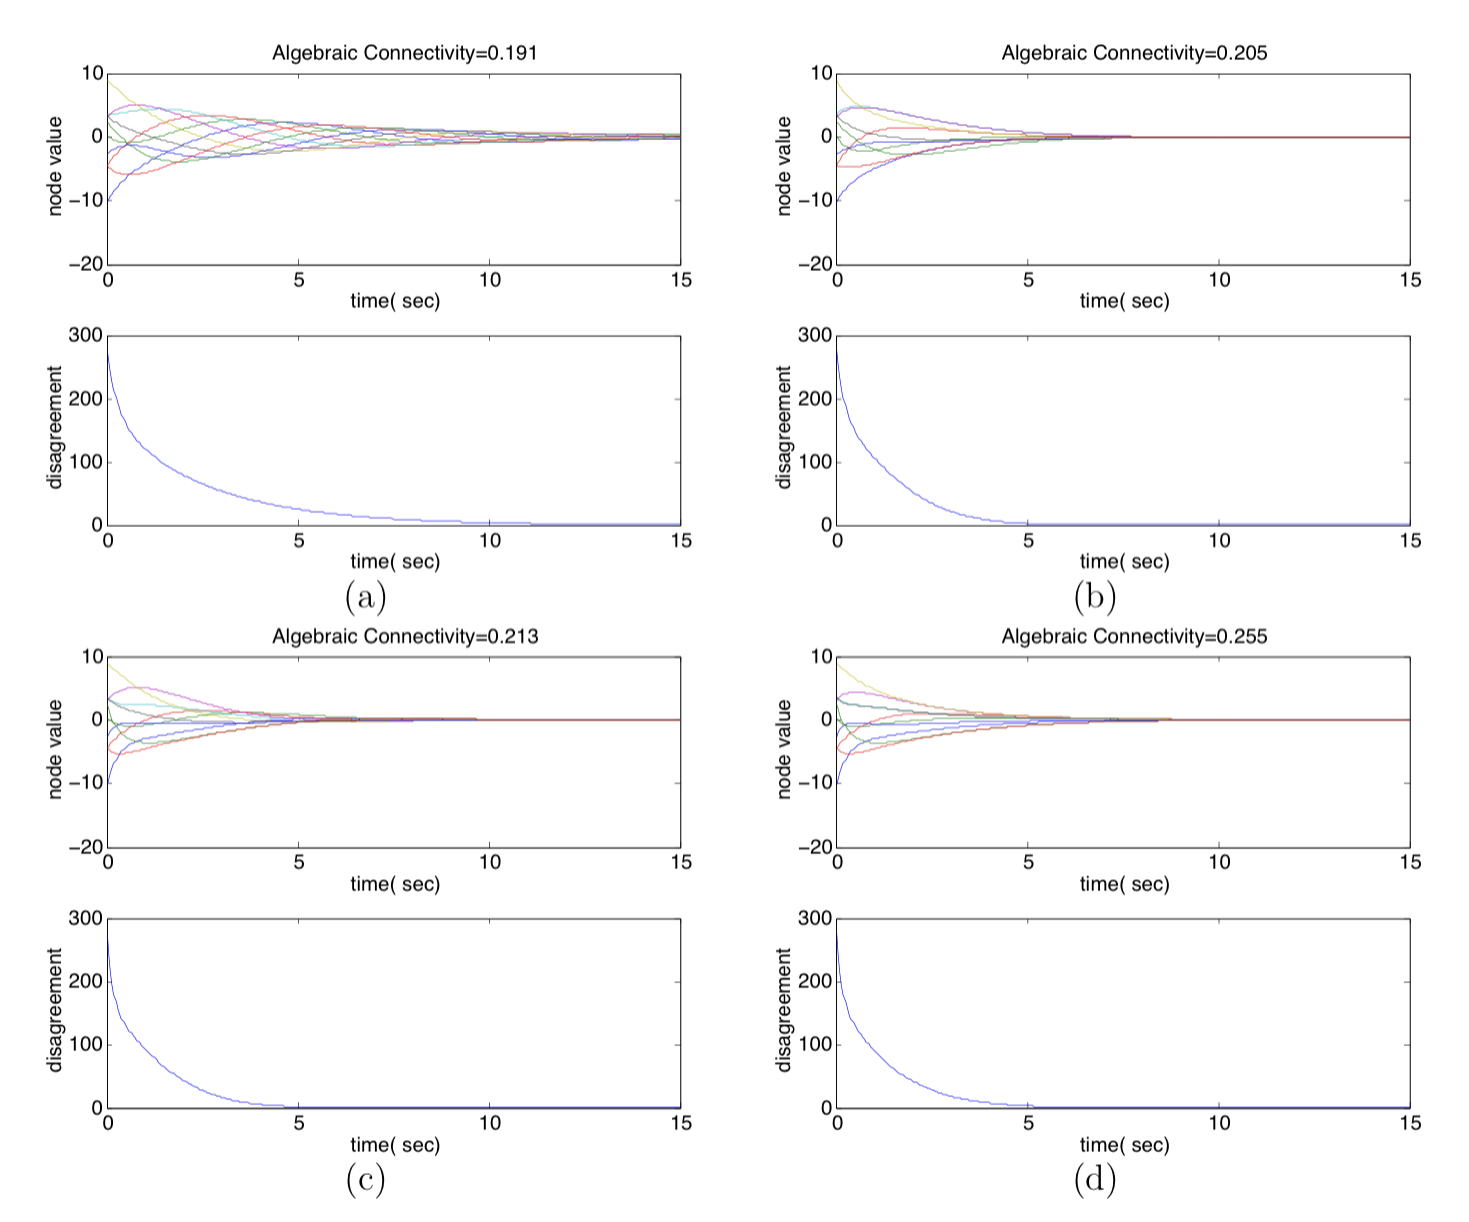
\includegraphics[width=14.5cm]{figures/Fig5-Simulation.jpeg}
    \label{Simulation}
    \caption{图的轨迹}
\end{figure}

在图6(a)中,一个有限自动机包含了状态集合\{$G_a, G_b, G_c, G_d$\},表示切换拓扑网络离散状态,作为一个混合系统。
这个混合系统从离散状态$G_b$开始,之后每经过$T=1$秒切换至图6(a)所示的下个状态。
网络的连续时间状态轨迹和群组非一致性(即$||\delta||^2$)如图6(b)所示。
清楚的看到,群组非一致性是单调递减的。
可以观看到平均一致性是逐渐达成的。
此外,群组非一致性呈指数级快速消失。
\begin{figure}[htbp]
    \centering
    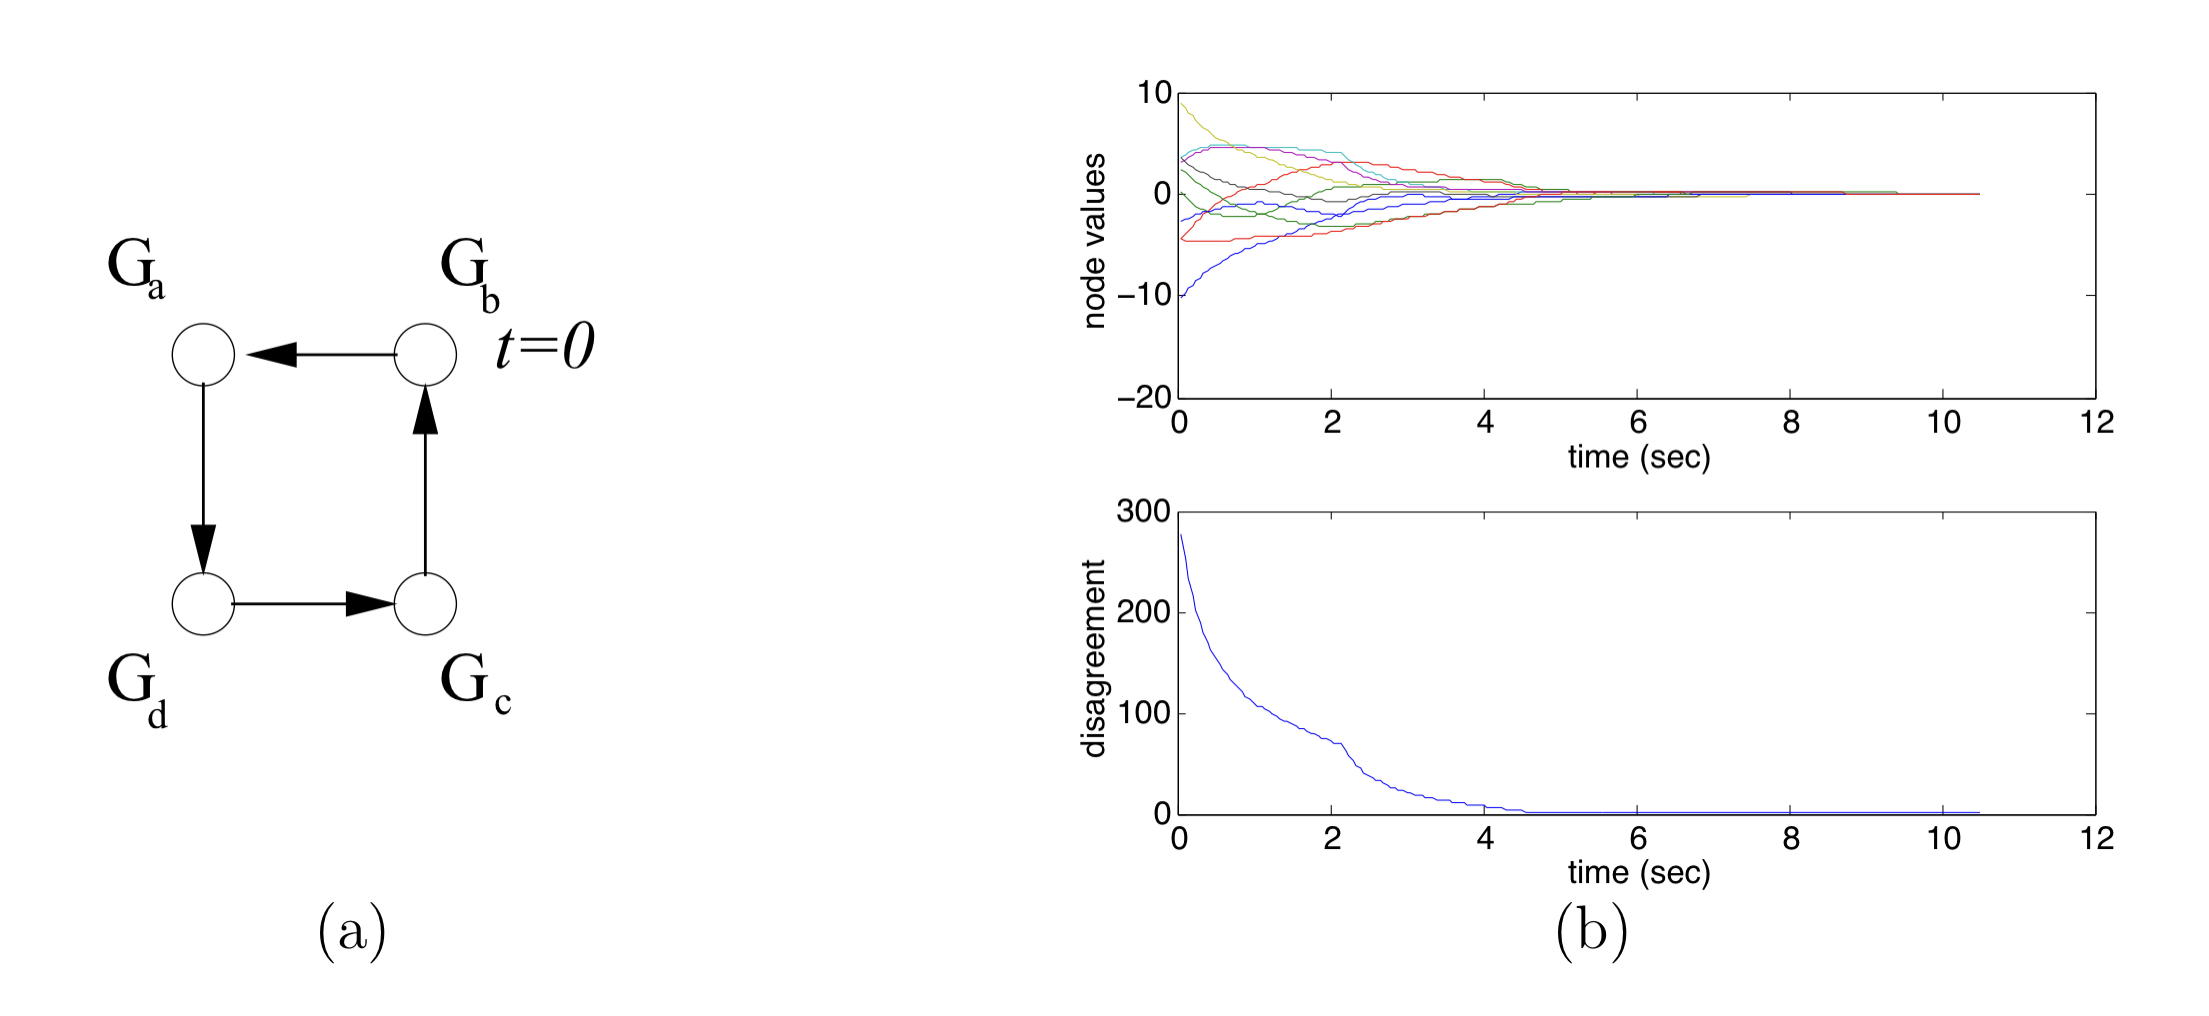
\includegraphics[width=14.5cm]{figures/Fig6-Automaton.jpeg}
    \label{Automaton}
    \caption{有限自动机}
\end{figure}

之后,我们展示了关于网络信息流的沟通时滞平均一致性问题的结果,如图7所示。
\begin{figure}[htbp]
    \centering
    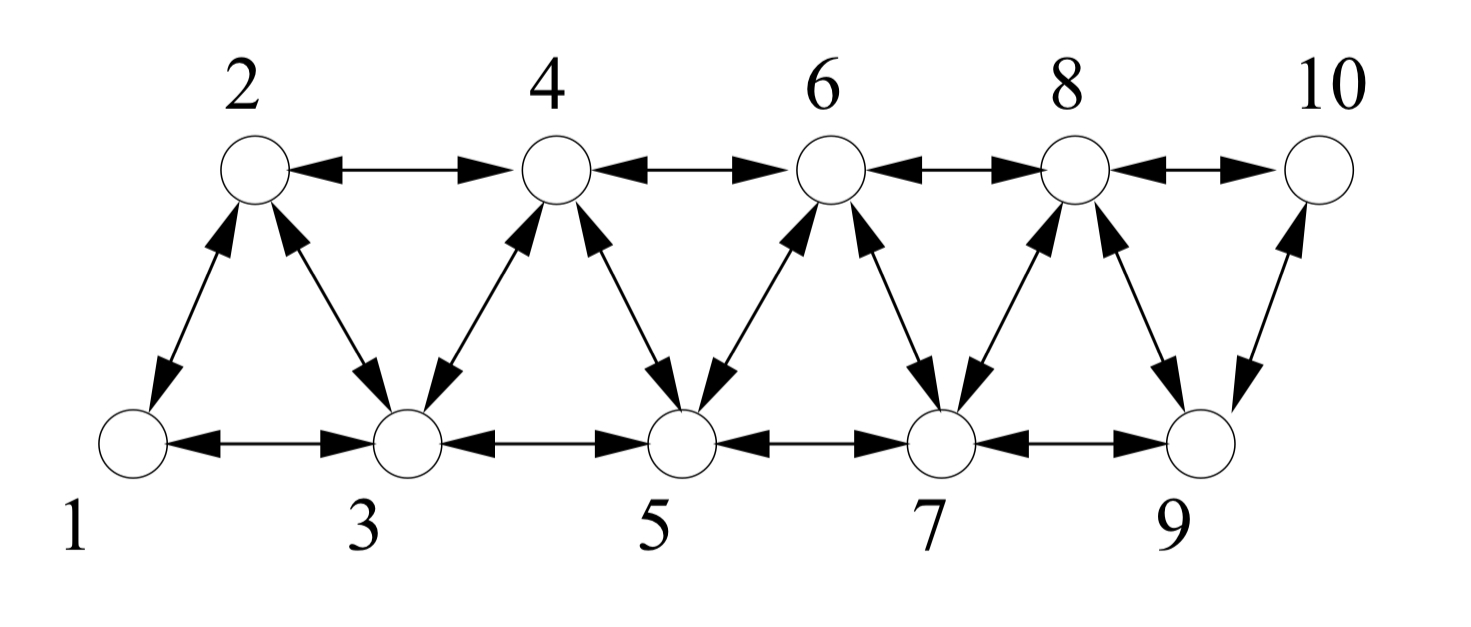
\includegraphics[width=8cm]{figures/Fig7-Undirected.jpeg}
    \label{Undirected}
    \caption{用作沟通时滞一致性的无向图$G_e$}
\end{figure}

图8展示了$n=10$网络节点状态轨迹,网络包含沟通时滞$\tau$,$\tau$的值有$\tau=0, 0.5\tau_{max}, \tau_{max} = \pi / 2\tau_{max}(G_a) = 0.266$,对于0均值随机初始条件的随机集合。
清楚的看到,当$\tau < \tau_{max}$时达到一致,如图8(a),(b)和(c)所示。
针对于$\tau = \tau_{max}$的情况,同步振荡如图8(d)所示。
三阶帕德近似(Pade approximation)被用在时滞模型作为一个有限阶线性时不变(Linear Time-Invariant, LTI)系统。


\section{Conclusions}
我们提供了具备有向信息流和固定或切换拓扑网络的一致性协议的收敛性分析。
我们的分析依赖于一些代数图论和矩阵论的工具。
我们建立了线性一致性协议的性质和镜像图拉普拉斯算子的费德勒特征值之间的联系。
介绍了简单的非一致性函数,其作为李雅普诺夫方程,允许切换拓扑网络的一致性协议的收敛性分析。
给出的交换图,该图表明了平衡图的加权邻接矩阵采用矩阵交换的拉普拉斯算子和对称部分矩阵的运算。
平衡图被证明对解决平均一致性问题是有帮助的。

对于无向图网络,我们给出了通信时滞网络一致性的充分必要条件。
这表明在时滞鲁棒性和线性一致性协议的收敛速度之间存在折中。
\begin{figure}[htbp]
    \centering
    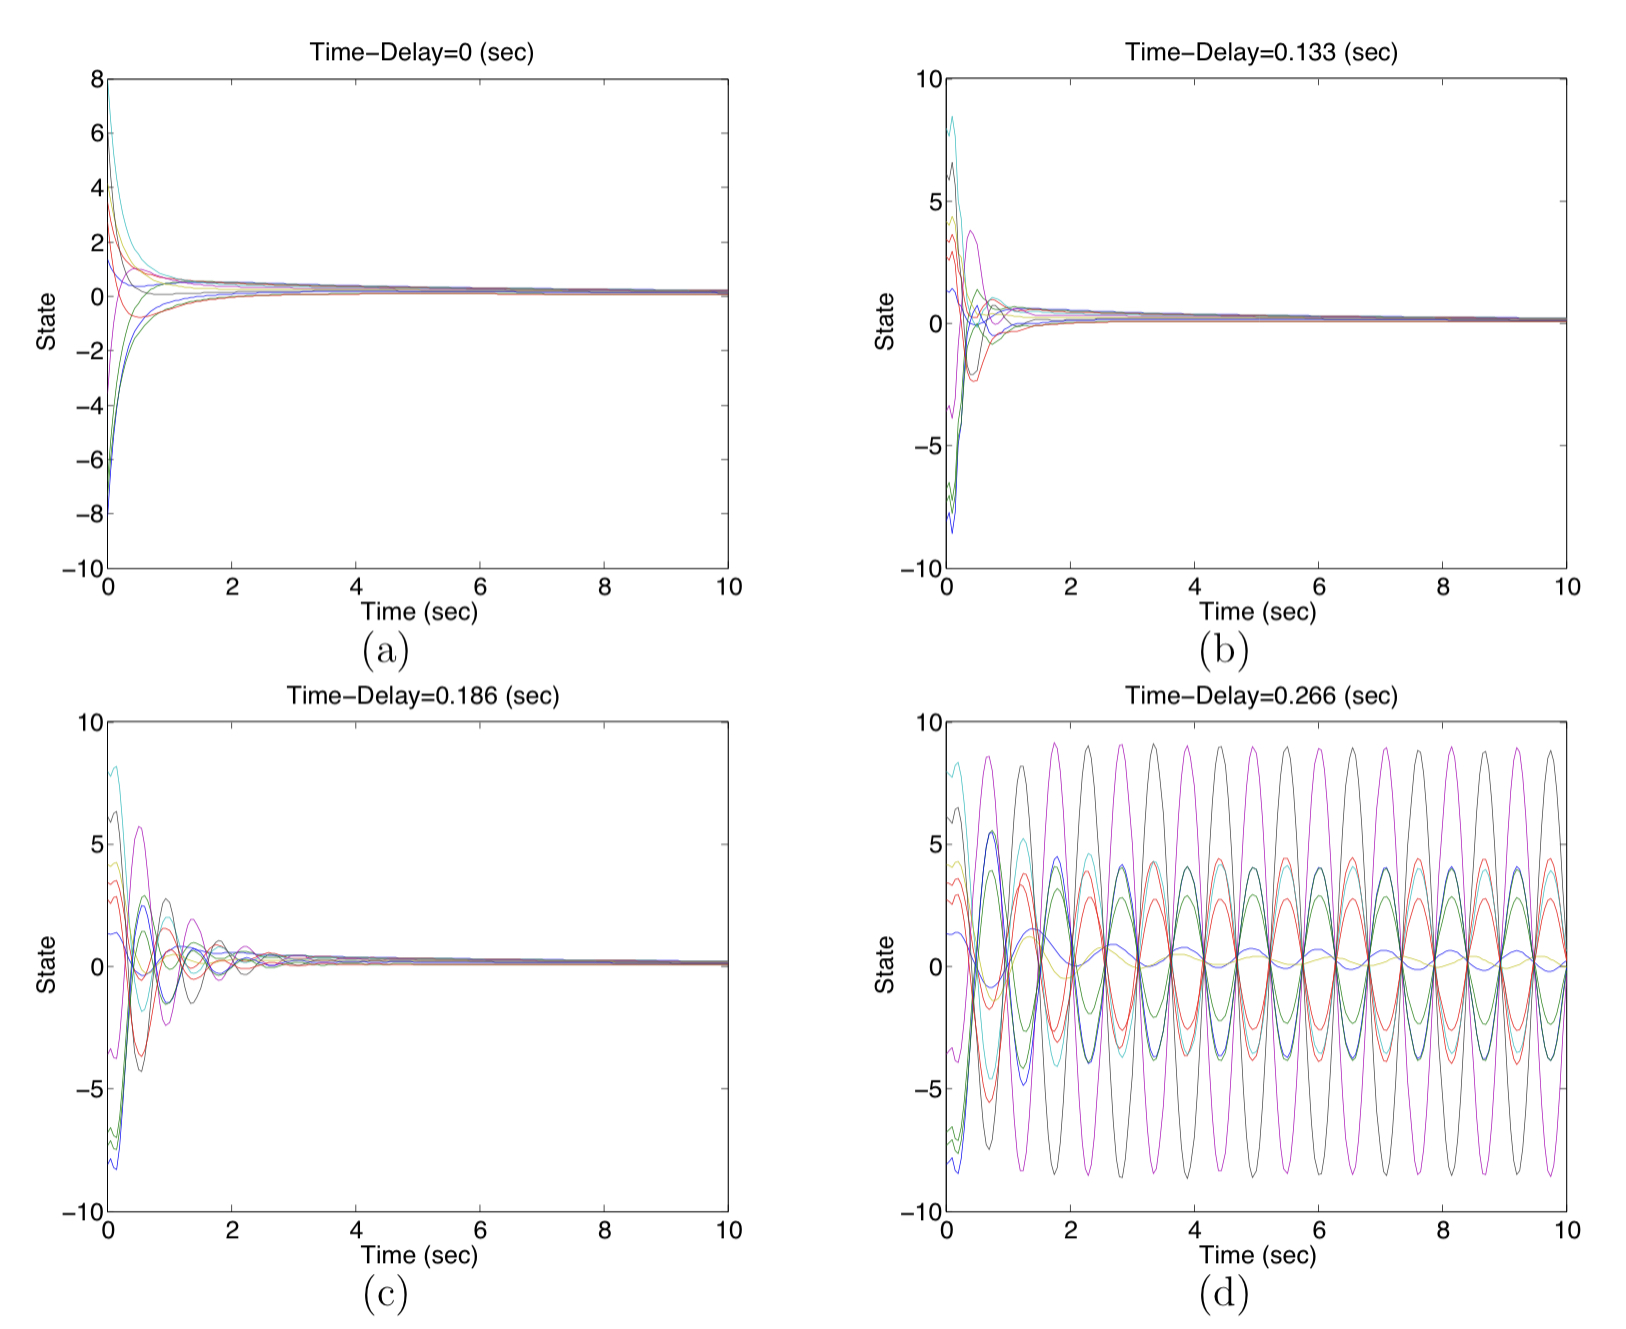
\includegraphics[width=14.5cm]{figures/Fig8-ConsensusProblem.jpeg}
    \label{ConsensusProblem}
    \caption{一致性问题}
\end{figure}

为了确定智能体群组的领导性问题,我们介绍了最大化智能体,它拥有一个简单的离散时间模型并且通过最大化的$n-1$次迭代($n$代表智能体的总数),给出了使用分布式方式解决最大一致性问题的协议。

我们提出了复杂的仿真结果以此演示了我们理论结果的有效性。

综合智能体离散时间渐进的一致性问题主要依赖非负矩阵理论,这将在下个文章中指出。

\end{document}